\chapter{Ensayos y Resultados}
\label{chap:ensayos_resultados}

El capítulo reúne las pruebas que validan la infraestructura desplegada en el Capítulo~\ref{chap:diseno_implementacion} frente a los objetivos funcionales, de seguridad, de rendimiento y de continuidad operativa definidos en la Sección~\ref{sec:objetivos_alcance}. Las verificaciones avanzan por capas: despliegue de cada servicio, integración entre componentes, control de acceso, flujo funcional completo, métricas de consumo de recursos y restauración de respaldos. Cada ensayo contrasta el comportamiento observado en producción contra el diseño previsto, y el capítulo cierra con una matriz de trazabilidad que vincula los requisitos con la evidencia obtenida.

\section{Metodología de Validación}
\label{sec:metodologia_validacion}

La validación abarca el comportamiento de los componentes desplegados, sus integraciones y el sistema en su conjunto bajo condiciones controladas de producción. Las verificaciones se organizan en cinco capas progresivas:

\begin{itemize}
    \item Capa de servicio: verificación de que cada contenedor inicia, supera su \textit{healthcheck} y mantiene disponibilidad en el tiempo.
    \item Capa de integración: verificación de que los canales de comunicación entre servicios retornan respuestas exitosas y no registran errores en producción (Documenso con PostgreSQL, Browserless, MinIO y el \textit{relay} SMTP de Brevo).
    \item Capa de sistema: ejecución del flujo de firma completo de extremo a extremo en producción, desde la carga del documento hasta la descarga del PDF sellado.
    \item Capa de rendimiento: observación del consumo de CPU y RAM durante operación normal y bajo carga controlada.
    \item Capa de continuidad: verificación de que los respaldos automáticos se almacenan correctamente y que un volcado puede restaurarse sin pérdida de datos.
\end{itemize}

Las herramientas empleadas para la recolección de evidencia fueron: la interfaz de Coolify (logs de contenedores y estado de servicios), las herramientas de desarrollo del navegador (trazas HTTP), Adobe Reader (validación de firma en PDF), Gmail (headers técnicos de autenticación SMTP) y Netdata (métricas de CPU y RAM por contenedor).

\section{Validación de Despliegue de Servicios}
\label{sec:validacion_despliegue}

Esta sección verifica que la capa de servicio descrita en la Sección~\ref{sec:metodologia_validacion} es operativa: cada contenedor del \textit{stack} alcanzó el estado \texttt{Healthy} y superó las pruebas de disponibilidad configuradas en el Capítulo~\ref{chap:diseno_implementacion}. La validación se presenta en dos niveles complementarios: la verificación de los \textit{healthchecks} a nivel de infraestructura desde la interfaz de Coolify y la consulta del \textit{endpoint} de diagnóstico interno de Documenso.

\subsection{Estado de los contenedores en Coolify}
\label{subsec:validacion_healthcheck}

El archivo de composición del despliegue, presentado en la Sección~\ref{sec:configuracion_servicios} del Capítulo~\ref{chap:diseno_implementacion}, define una directiva \texttt{healthcheck} para cada servicio del \textit{stack}. Las Figuras~\ref{fig:coolify_healthy_main} y \ref{fig:coolify_healthy_socat} reflejan visualmente la resolución exitosa del árbol de dependencias del orquestador (\textit{depends\_on}) y la confirmación de los \textit{healthchecks} internos: los servicios \texttt{documenso}, \texttt{database}, \texttt{browserless} y \texttt{socat} se observan en estado \texttt{Healthy}, en coherencia con el diseño de despliegue.

\begin{figure}[!htbp]
    \centering
    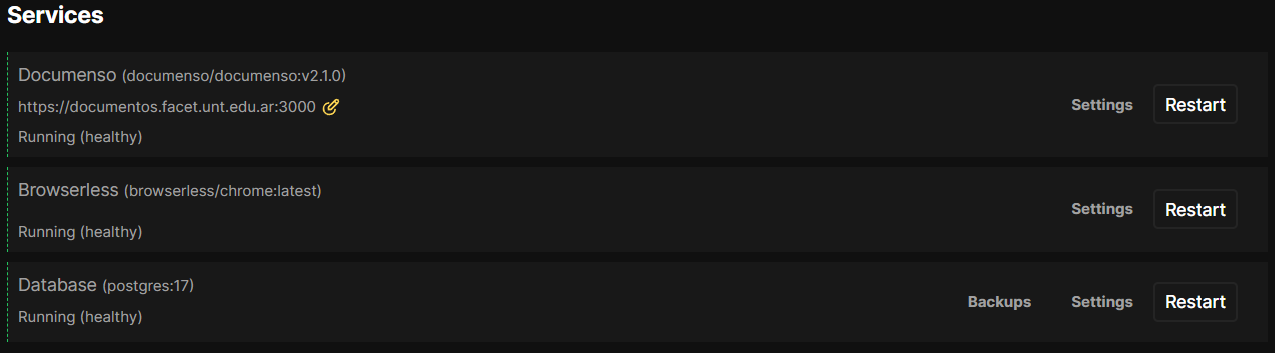
\includegraphics[width=\textwidth]{figuras/capitulo4/4.2/documenso_browserless_database_healthyOnCoolify.png}
    \caption[Panel de Coolify: servicios principales en estado Healthy]{Evidencia del estado \texttt{Healthy} de los servicios \texttt{documenso}, \texttt{database} y \texttt{browserless}, consistente con la resolución de dependencias y la ejecución satisfactoria de \textit{healthchecks} internos.}
    \label{fig:coolify_healthy_main}
\end{figure}

\begin{figure}[!htbp]
    \centering
    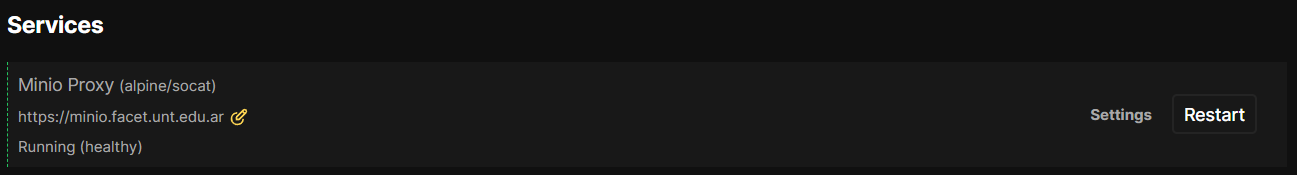
\includegraphics[width=\textwidth]{figuras/capitulo4/4.2/socat_healthyOnCoolify.png}
    \caption[Panel de Coolify: servicio Socat en estado Healthy]{Evidencia del estado \texttt{Healthy} del servicio \texttt{socat}, consistente con la validación operativa del \textit{proxy} TCP hacia MinIO en el puerto 9000.}
    \label{fig:coolify_healthy_socat}
\end{figure}

\FloatBarrier

El estado \texttt{Healthy} de los cuatro servicios confirma que el \textit{stack} completo superó sus pruebas de disponibilidad. Dado que \texttt{documenso} declara \texttt{depends\_on} sobre \texttt{database} con la condición \texttt{service\_healthy}, su propio estado \texttt{Healthy} implica además que PostgreSQL completó sus verificaciones antes de que la aplicación iniciara.

\subsection{Verificación del estado interno de la aplicación}
\label{subsec:validacion_api_health}

Documenso expone además el endpoint \texttt{/api/health}, que extiende la verificación de infraestructura hacia los subsistemas internos de la aplicación. A diferencia del \textit{healthcheck} de Docker —que únicamente comprueba accesibilidad de red—, este \textit{endpoint} reporta el estado de la conectividad con la base de datos y la disponibilidad del certificado de firma.

El Código~\ref{lst:api_health_response} muestra la respuesta obtenida al consultar \nolinkurl{https://documentos.facet.unt.edu.ar/api/health}.

\begin{lstlisting}[caption={Respuesta del endpoint \texttt{/api/health} de Documenso}, label={lst:api_health_response}]
{
  "status": "ok",
  "timestamp": "2026-04-12T15:01:14.367Z",
  "checks": {
    "database":    { "status": "ok" },
    "certificate": { "status": "ok" }
  }
}
\end{lstlisting}

Los tres campos con valor \texttt{ok} confirman que la aplicación está operativa, que Documenso estableció conectividad con PostgreSQL y que el certificado de firma institucional está cargado y disponible.

\FloatBarrier

\section{Verificación de la Comunicación entre Servicios}
\label{sec:verificacion_comunicacion}

Esta sección valida que los canales de comunicación entre los componentes del despliegue operan según el diseño descrito en el Capítulo~\ref{chap:diseno_implementacion}, mediante tres verificaciones: la conectividad con el almacenamiento de objetos MinIO a través del \textit{proxy} Socat, la comunicación con Browserless para el renderizado del certificado de firma y la entregabilidad del correo transaccional a través del \textit{relay} de Brevo.

\subsection{Conectividad con el almacenamiento de objetos (MinIO)}
\label{subsec:validacion_minio}

Los logs HTTP del servidor MinIO registran los dos flujos de acceso al \textit{bucket} \texttt{documenso-prod}: el directo, originado desde el navegador del usuario, y el indirecto, originado desde el \textit{backend} de la aplicación.

La Figura~\ref{fig:minio_log_flujo_directo} muestra una operación \texttt{PUT 200 OK} cuyo campo \texttt{User-Agent} identifica al cliente como un navegador Microsoft Edge con IP de origen externa a la red institucional, lo que confirma que la solicitud atravesó el recorrido completo: \textit{reverse proxy} perimetral, Traefik, contenedor Socat y servidor físico TrueNAS.

\begin{figure}[!htbp]
    \centering
    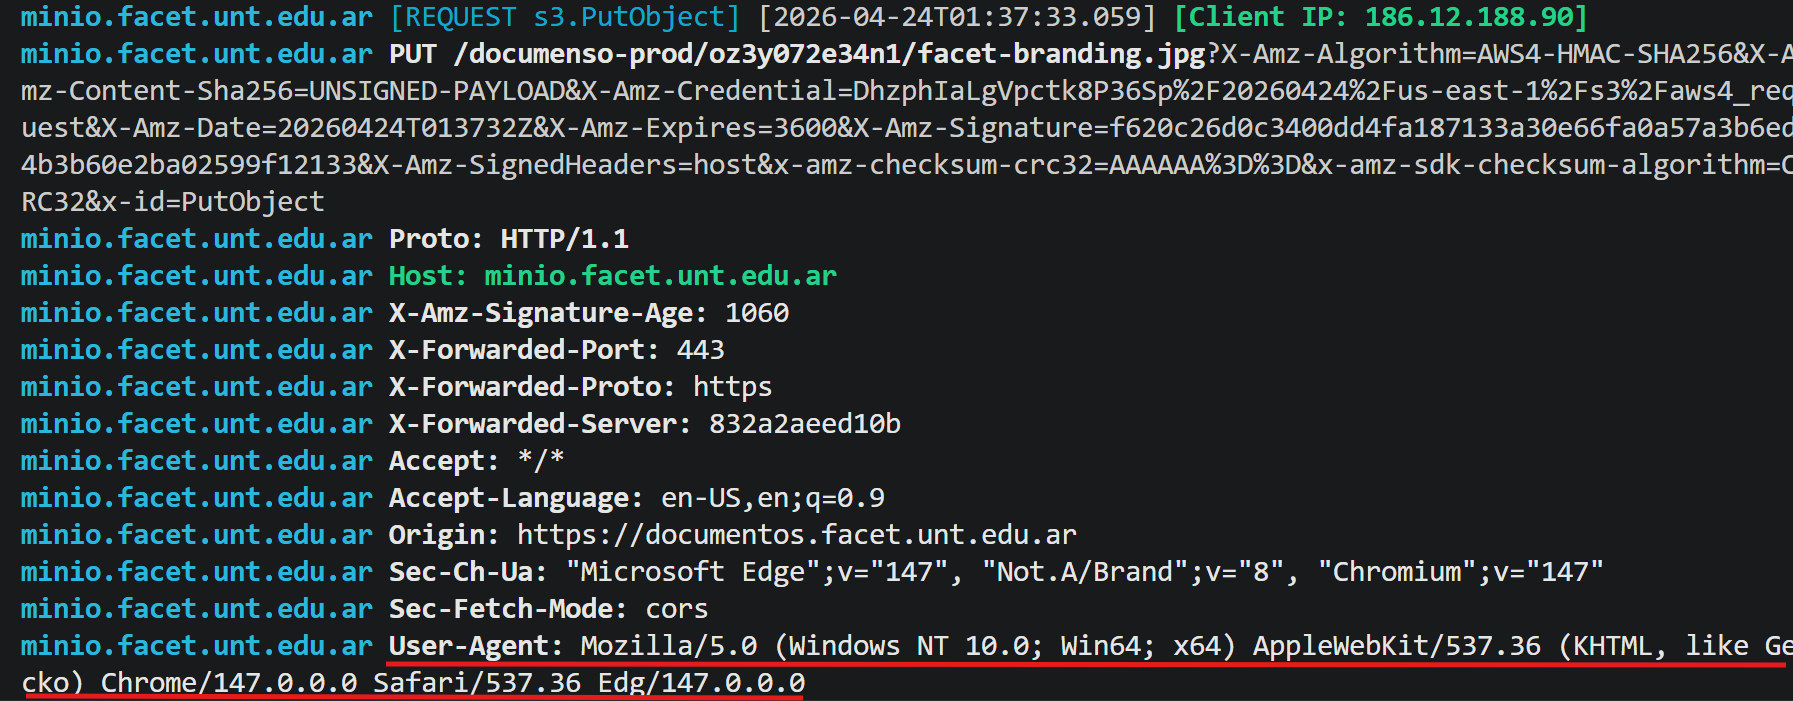
\includegraphics[width=\textwidth]{figuras/capitulo4/4.3/minio_logs_flujo_directo.png}
    \caption[Registro de acceso HTTP de MinIO: flujo directo desde el navegador]{Registro de acceso HTTP del servidor MinIO mostrando una operación \texttt{PUT 200 OK} originada desde un navegador Microsoft Edge. El campo \texttt{User-Agent} identifica el flujo directo documentado en la Sección~\ref{sec:proxy_socat}.}
    \label{fig:minio_log_flujo_directo}
\end{figure}

La Figura~\ref{fig:minio_log_flujo_indirecto} muestra el registro de una operación \texttt{GET} con código \texttt{200 OK} sobre ese bucket. En este caso, el campo \texttt{User-Agent} indica \texttt{node}, lo que identifica al cliente como el proceso Node.js del \textit{backend} de Documenso. Este registro corresponde al flujo indirecto: la aplicación recupera el documento PDF desde MinIO a través del \textit{proxy} Socat para procesarlo internamente.

\begin{figure}[!htbp]
    \centering
    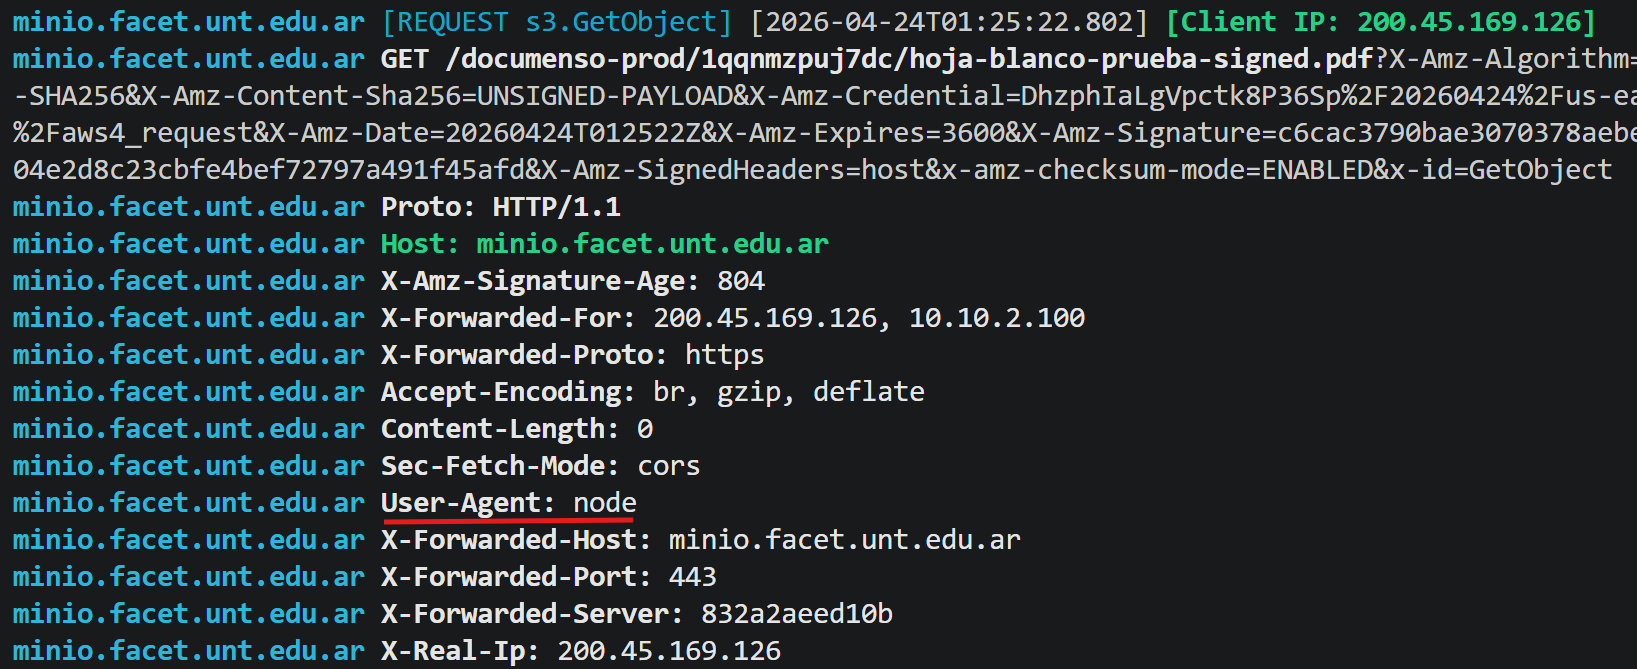
\includegraphics[width=\textwidth]{figuras/capitulo4/4.3/minio_logs_flujo_indirecto.png}
    \caption[Registro de acceso HTTP de MinIO: flujo indirecto desde el \textit{backend}]{Registro de acceso HTTP del servidor MinIO mostrando una operación \texttt{GET 200 OK} con \texttt{User-Agent: node}. El identificador confirma que el cliente es el proceso \textit{backend} de Documenso, correspondiente al flujo indirecto.}
    \label{fig:minio_log_flujo_indirecto}
\end{figure}

\FloatBarrier

Ambos registros, observados desde el servidor de almacenamiento, confirman que los dos flujos definidos en el diseño operan correctamente en producción: el canal directo navegador-MinIO y el canal indirecto backend-MinIO reciben respuestas \texttt{200 OK} del servidor, lo que valida la cadena completa de conectividad a través del proxy Socat.

\subsection{Comunicación con Browserless (renderizado del certificado de firma)}
\label{subsec:validacion_browserless}

Los registros de los contenedores \texttt{documenso} y \texttt{browserless} se analizaron para verificar que el renderizado del certificado de firma opera sin errores en producción.

El Código~\ref{lst:documenso_seal_trigger} contiene el fragmento de los registros de Documenso al momento en que se disparó el job de sellado para el documento~12.

\begin{lstlisting}[caption={Registros del contenedor Documenso: disparo del job \texttt{internal.seal-document}}, label={lst:documenso_seal_trigger}, breaklines=true]
2026-Apr-11 17:48:46
[JOBS]: Triggering job internal.seal-document with payload
{ documentId: 12, requestMetadata: { ipAddress: '148.222.222.66',
  userAgent: 'Mozilla/5.0 (Windows NT 10.0; Win64; x64) ...' } }
2026-Apr-11 17:48:46
Submitting job to endpoint:
http://documenso:3000/api/jobs/internal.seal-document/[JOB_ID]
\end{lstlisting}

El Código~\ref{lst:browserless_seal_success} registra la respuesta de Browserless, comprendida entre los instantes 17:48:52 y 17:49:11 UTC.

\pagebreak
\begin{lstlisting}[caption={Registros del contenedor Browserless: recepción y completado del job de renderizado}, label={lst:browserless_seal_success}]
17:48:52 browserless:job    [...]: Inbound WebSocket request.
17:48:52 browserless:job    [...]: Adding new job to queue.
17:48:52 browserless:system Generating fresh chrome browser
17:48:52 browserless:chrome-helper Launching Chrome with args:
         { "executablePath": "/usr/bin/google-chrome" }
17:49:06 browserless:system Got chrome instance
17:49:11 browserless:server [...]: Recording successful stat
                                    and cleaning up.
17:49:11 browserless:chrome-helper Browser process [...] has
                      closed, cleaning up.
\end{lstlisting}

\FloatBarrier

Los registros evidencian que Browserless recibió la solicitud de renderizado por WebSocket, lanzó una instancia de Chrome desde \texttt{/usr/bin/google-chrome} y completó el procesamiento en aproximadamente 18~segundos. El mensaje \texttt{Recording successful stat and cleaning up} confirma que el job concluyó sin errores. Este resultado confirma que la limitación documentada en la Subsección~\ref{subsec:browserless} del Capítulo~\ref{chap:diseno_implementacion} quedó resuelta en producción y que el sellado criptográfico del documento puede completarse.

\FloatBarrier

\subsection{Entregabilidad del correo transaccional (Brevo SMTP)}
\label{subsec:validacion_smtp}

La Figura~\ref{fig:smtp_auth_headers} presenta la evidencia recolectada en Gmail mediante la inspección de encabezados SMTP de un correo transaccional emitido por Documenso, donde se observan los mecanismos SPF, DKIM y DMARC. Estos resultados (\texttt{PASS}) garantizan que los proveedores de correo reconozcan la legitimidad de las notificaciones emitidas por la plataforma. En la práctica, esto evita que los avisos de firma sean bloqueados o marcados como \textit{spam},

\begin{figure}[!htbp]
    \centering
    \colorbox{black}{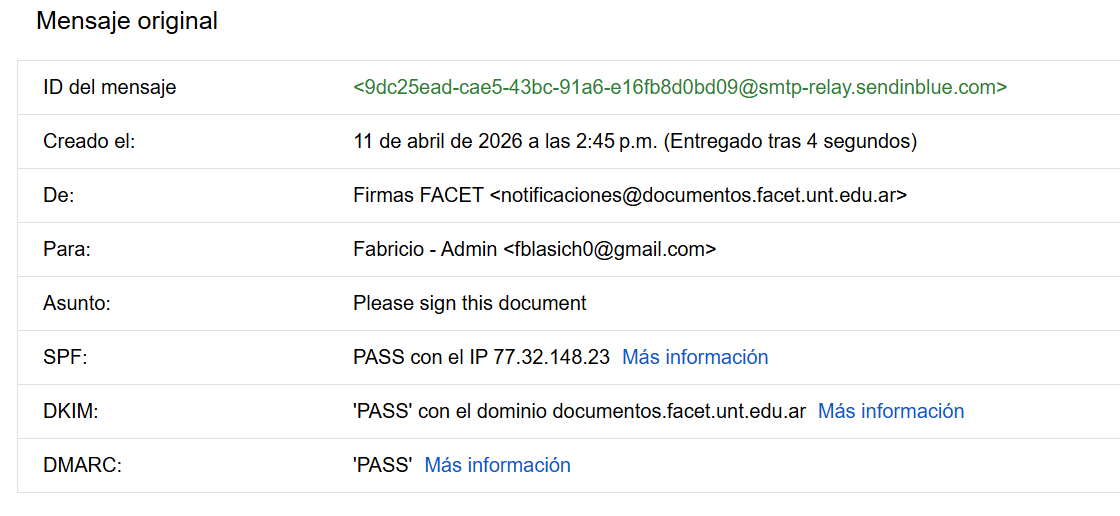
\includegraphics[width=0.85\textwidth]{figuras/capitulo4/4.3/headers_mail.png}}
    \caption[Encabezados de autenticación SMTP de un correo transaccional de Documenso]{Captura de encabezados SMTP obtenida en Gmail para un correo transaccional de Documenso. Se visualizan los resultados de validación de SPF, DKIM y DMARC sobre el mensaje emitido a través del \textit{relay} de Brevo.}
    \label{fig:smtp_auth_headers}
\end{figure}

\FloatBarrier

\section{Validación de Acceso y Control de Seguridad}
\label{sec:validacion_acceso}

Esta sección verifica que el mecanismo de acceso a la plataforma opera según lo configurado en la Subsección~\ref{subsec:google_oauth}: solo cuentas pertenecientes al dominio institucional pueden autenticarse, y el registro libre de nuevos usuarios está deshabilitado.

\subsection{Restricción del inicio de sesión con Google OAuth 2.0}
\label{subsec:validacion_oauth}

Al intentar iniciar sesión con una cuenta externa al dominio institucional, Google interrumpió el flujo de OAuth antes de emitir el código de autorización: el servidor de autorización devolvió el código \texttt{Error 403: org\_internal} con el mensaje \texttt{Acceso bloqueado: Sistema\allowbreak FirmasFACET solo se puede usar dentro de su organización} (Figura~\ref{fig:oauth_error_gmail}). Este comportamiento es consecuencia directa de haber configurado el tipo de aplicación como \textit{Interna} en Google Cloud Console, tal como se describió en la Subsección~\ref{subsec:google_oauth}: la restricción opera en la capa de autorización de Google y no depende de ninguna validación adicional por parte de la aplicación.

\begin{figure}[!htbp]
    \centering
    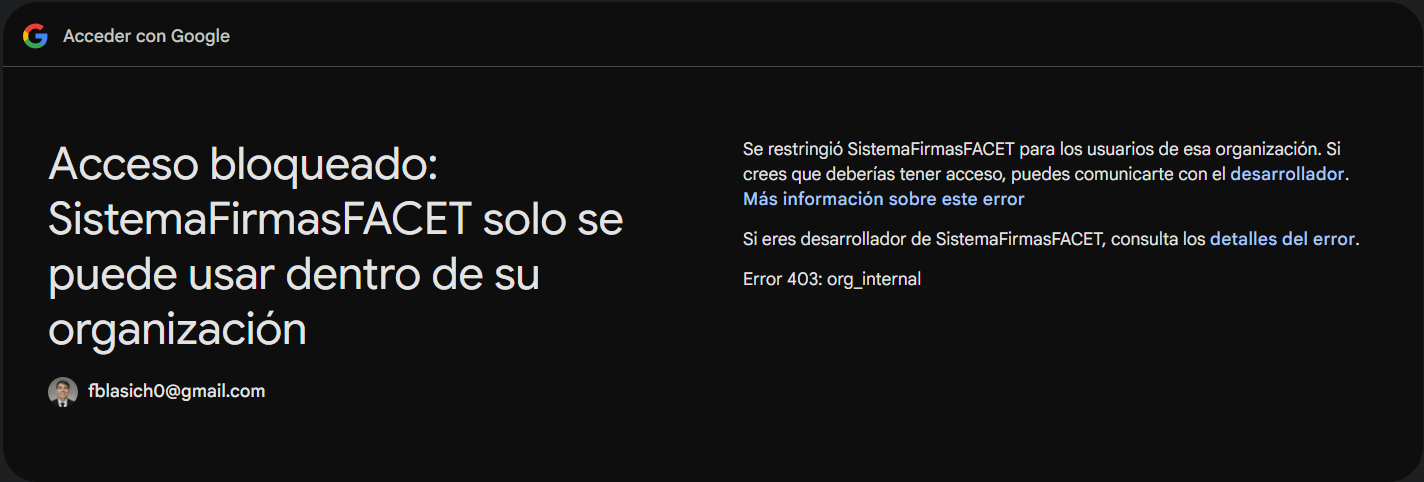
\includegraphics[width=0.92\textwidth]{figuras/capitulo4/4.4/oauth_flow_gmail.png}
    \caption[Error de acceso con cuenta externa en Google OAuth]{Pantalla de error devuelta por Google al intentar autenticarse con una cuenta \texttt{@gmail.com}. El código \texttt{org\_internal} confirma que la restricción opera en la capa de autorización de Google.}
    \label{fig:oauth_error_gmail}
\end{figure}

Con una cuenta \texttt{@herrera.unt.edu.ar}, Google presentó el modal de consentimiento y, una vez aceptado, el servidor emitió el código de autorización; el backend de Documenso completó el intercambio y el usuario accedió al panel de trabajo.

\FloatBarrier

\subsection{Deshabilitación del registro local}
\label{subsec:validacion_signup}

El registro de usuarios mediante credenciales locales fue deshabilitado a través de la variable de entorno \texttt{NEXT\_PUBLIC\_DISABLE\_SIGNUP=true}, cuyo efecto en la interfaz se documentó en la Subsección~\ref{subsec:google_oauth} (Figura~\ref{fig:google_oauth_disable_signup}).

Se realizó una solicitud GET directa a \nolinkurl{https://documentos.facet.unt.edu.ar/signup} para verificar que la restricción opera a nivel de servidor. La solicitud retornó \texttt{302 Found} con \texttt{Location: /signin} (Figura~\ref{fig:signup_redirect_302}): la redirección es forzada por el backend antes de renderizar cualquier contenido de registro, lo que confirma que la restricción opera en la lógica de enrutamiento del servidor y no se limita a ocultar el formulario en el frontend.

\begin{figure}[!htbp]
    \centering
    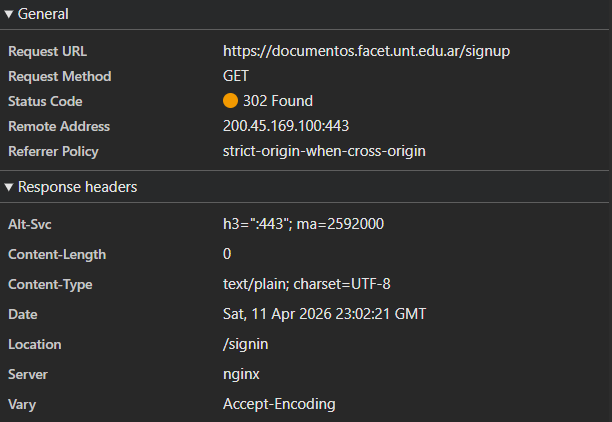
\includegraphics[width=0.75\textwidth]{figuras/capitulo4/4.4/request_endpoint_signup_302http.png}
    \caption[Respuesta HTTP 302 al acceder a la ruta \texttt{/signup}]{Captura de las herramientas de desarrollo del navegador mostrando la respuesta \texttt{302 Found} con redirección a \texttt{/signin} al intentar acceder directamente a la ruta de registro.}
    \label{fig:signup_redirect_302}
\end{figure}

\FloatBarrier

\section{Validación del Flujo Funcional de Extremo a Extremo}
\label{sec:validacion_e2e}
\label{sec:ensayos_validacion}

Esta sección valida la capa de sistema definida en la Sección~\ref{sec:metodologia_validacion}: el flujo completo de firma documental se ejecutó en producción con dos firmantes. La validación se presenta en dos partes: el ciclo operativo de extremo a extremo y la verificación de la firma electrónica incrustada en el documento resultante.

\subsection{Ciclo completo de firma documental}
\label{subsec:ciclo_e2e}

Se ejecutó un ciclo completo de firma sobre el documento \texttt{ejemplo1.pdf} con dos destinatarios: una cuenta institucional (\texttt{@herrera.unt.edu.ar}) y una cuenta externa al dominio (\texttt{@\allowbreak gmail.com}). El flujo recorrió las etapas de carga del documento, asignación de firmantes, posicionamiento de campos, notificación por correo electrónico y aplicación de la firma. El destinatario externo accedió mediante el enlace recibido por correo y completó la acción sin requerir cuenta local en la plataforma, lo que confirmó la operación del acceso por enlace documentado en la Subsección~\ref{subsec:google_oauth}. Al completarse ambas firmas, la plataforma disparó el job de sellado criptográfico descrito en la Subsección~\ref{subsec:validacion_browserless} y el ciclo concluyó sin errores.

El procedimiento paso a paso de este ciclo completo se documenta en el Apéndice~\ref{AppendixD}.

La Figura~\ref{fig:e2e_cierre} registra el cierre del ciclo. Al completarse ambas firmas, la plataforma emitió el correo de notificación con el PDF firmado adjunto y persistió el artefacto \texttt{\_signed.pdf} en el bucket \texttt{documenso-prod} de MinIO. Esta persistencia cerró el ciclo de integración validado en la Sección~\ref{sec:verificacion_comunicacion}: el documento sellado criptográficamente quedó almacenado en el bucket verificado en la Subsección~\ref{subsec:validacion_minio}.

\begin{figure}[t]
    \centering
    \begin{subfigure}[b]{0.60\textwidth}
        \centering
        \colorbox{black}{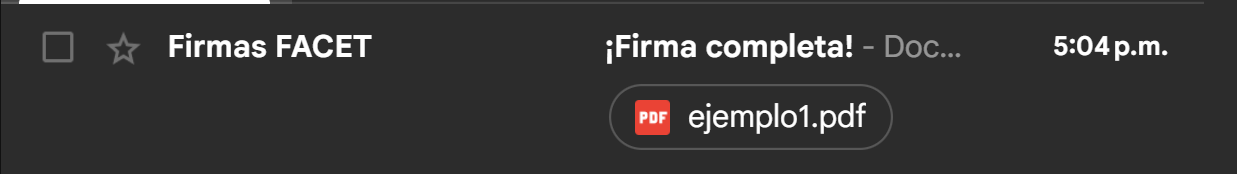
\includegraphics[width=\textwidth]{figuras/capitulo4/4.5/mail_documento_completado.png}}
        \caption{Correo de notificación de completado con PDF firmado adjunto.}
        \label{fig:e2e_mail_comp}
    \end{subfigure}
    \vspace{0.5em}
    \begin{subfigure}[b]{0.90\textwidth}
        \centering
        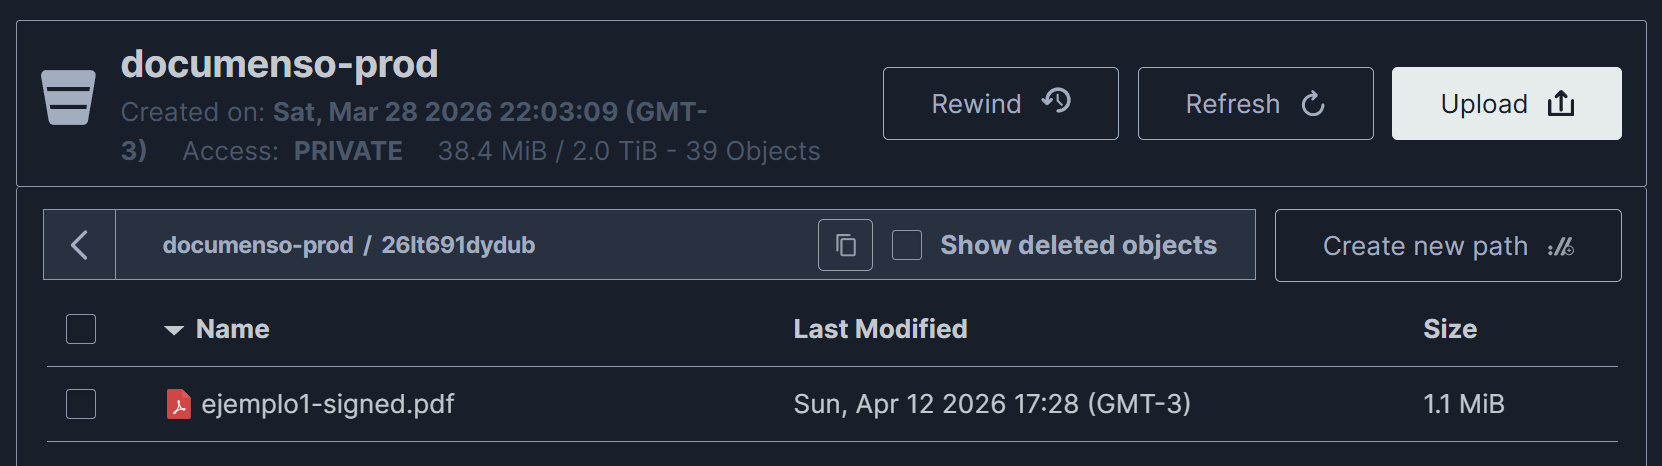
\includegraphics[width=\textwidth]{figuras/capitulo4/4.5/signedDocument_uploadToMinio.png}
        \caption{\textit{Bucket} \texttt{documenso-prod}: artefacto \texttt{\_signed.pdf} persistido en MinIO.}
        \label{fig:e2e_minio_signed}
    \end{subfigure}
    \caption[Cierre del ciclo de firma: notificación de completado y persistencia en MinIO]{Correo de notificación emitido al concluir el ciclo con el PDF firmado adjunto~(A); registro del artefacto \texttt{\_signed.pdf} en el \textit{bucket} \texttt{documenso-prod} de MinIO~(B).}
    \label{fig:e2e_cierre}
\end{figure}

\FloatBarrier

\subsection{Verificación de la firma electrónica en el documento}
\label{subsec:verificacion_firma_adobe}

El PDF descargado al concluir el ciclo documentado en la Subsección~\ref{subsec:ciclo_e2e} se analizó en Adobe Acrobat para confirmar que el sellado criptográfico realizado por Documenso es verificable desde un visor estándar.

El panel de firmas (Figura~\ref{fig:adobe_panel_firmas}) indica que no hubo modificaciones en el documento desde que se firmó; la advertencia de validez desconocida responde a que el certificado es autofirmado y no pertenece a una cadena de confianza comercial, comportamiento previsto en el diseño y documentado en la Subsección~\ref{sec:mecanismo_tecnico}.

\begin{figure}[!htbp]
    \centering
    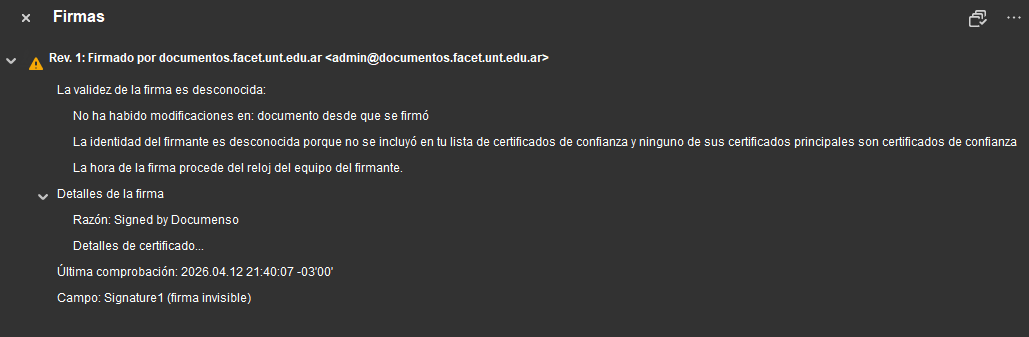
\includegraphics[width=0.88\textwidth]{figuras/capitulo4/4.5/panel_firmas_adobe.png}
    \caption[Panel de firmas en Adobe Acrobat sobre el documento sellado]{Panel de firmas de Adobe Acrobat. Se indica que no hubo modificaciones en el documento desde que se firmó y se identifican los detalles del firmante institucional.}
    \label{fig:adobe_panel_firmas}
\end{figure}

La Figura~\ref{fig:adobe_visor_cert} detalla el certificado utilizado: emisor y sujeto son documentos.facet.unt.edu.ar (FACET), con vigencia del 28/03/2026 al 25/03/2036. Este intervalo corresponde al parámetro \texttt{-days 3650} utilizado en la generación del certificado. La concordancia entre la vigencia exhibida por Microsoft Edge y el parámetro de generación confirma que el visor reconoce el material criptográfico institucional producido durante el despliegue (Apéndice~\ref{AppendixB:Crypto}).

\begin{figure}[!htbp]
    \centering
    \colorbox{black}{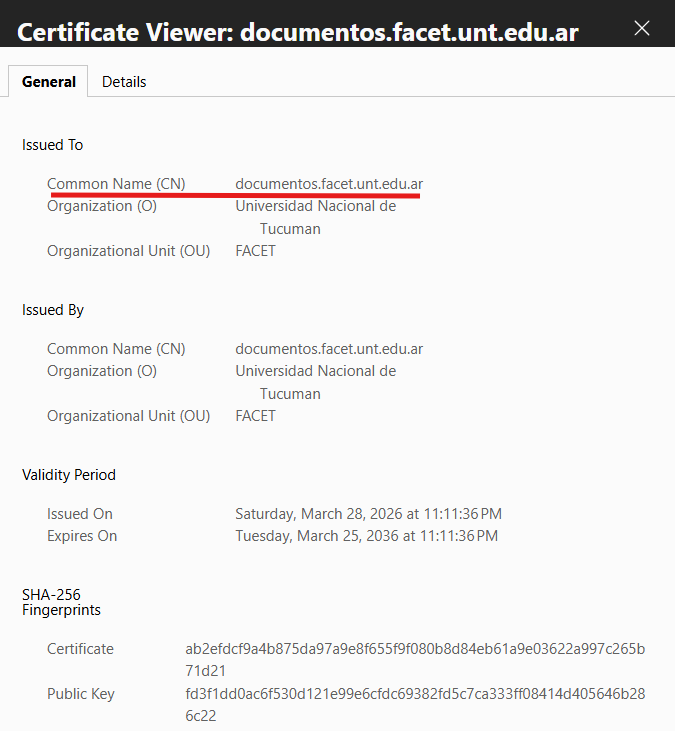
\includegraphics[width=0.80\textwidth]{figuras/capitulo4/4.5/visor_certificados_adobe.png}}
    \caption[Detalle del certificado institucional FACET en el visor de Microsoft Edge]{Visor de certificados de Microsoft Edge. Emisor y sujeto son \texttt{documentos.facet.unt.edu.ar} (FACET); vigencia del 28/03/2026 al 25/03/2036.}
    \label{fig:adobe_visor_cert}
\end{figure}

\FloatBarrier

\section{Métricas de Rendimiento del Sistema}
\label{sec:metricas_rendimiento}

Las métricas de consumo de CPU y RAM se registraron por contenedor mediante Netdata. Los valores se contrastan a continuación con la capacidad auditada del LXC: 8~vCPUs y 8~GiB de RAM (Subsección~\ref{sec:infraestructura_base}). En todas las gráficas de esta sección, la curva amarilla corresponde a Documenso, la naranja a Browserless, la azul a PostgreSQL y la rosa al \textit{proxy} Socat.

\subsection{Consumo de recursos en operación normal (baseline)}
\label{subsec:baseline}

El baseline se registró el 13 de abril de 2026 entre las 21:44 y las 22:00 UTC bajo condiciones de navegación estándar y descarga de archivos, sin ejecución de ciclos de firma concurrentes.

\subsubsection*{Memoria RAM}

La Figura~\ref{fig:baseline_ram} registra el consumo de RAM de los cuatro contenedores del \textit{stack} durante el período de observación. Las curvas se mantuvieron planas a lo largo del período, lo que descartó fugas de memoria en operación normal.

\begin{figure}[!htbp]
    \centering
    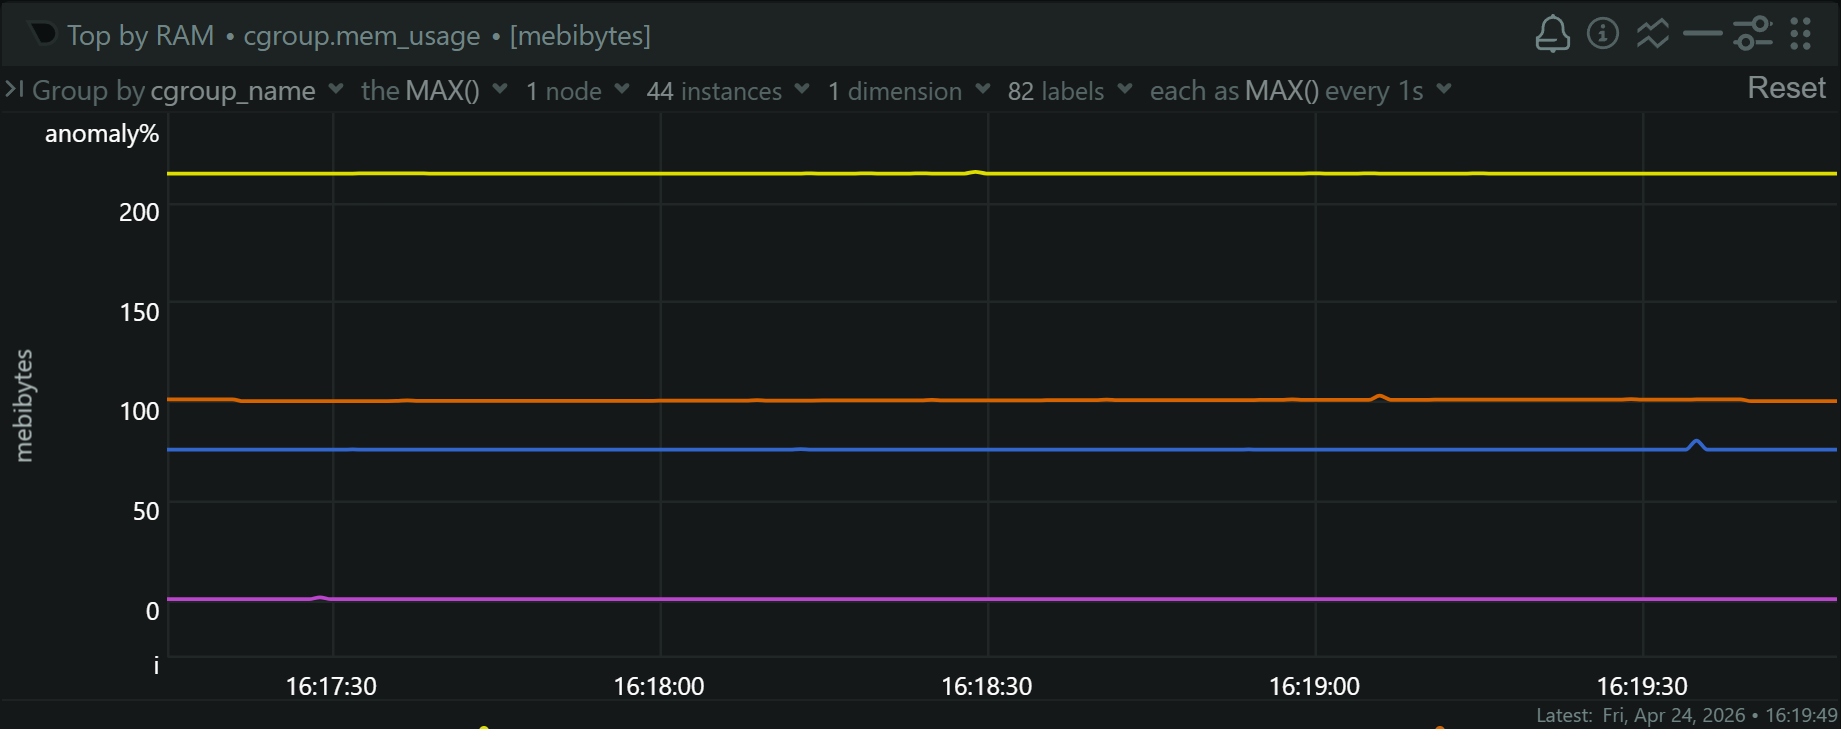
\includegraphics[width=\textwidth]{figuras/capitulo4/4.6/BloqueA/baseline_ram.png}
    \caption[Consumo de RAM en baseline: cuatro contenedores del \textit{stack}]{Consumo de RAM (en MiB) de los contenedores del \textit{stack} durante parte del período de observación en baseline. Documenso: \(\approx\) 215,5~MiB; Browserless: \(\approx\) 102,0~MiB; PostgreSQL: \(\approx\) 77,0~MiB; \textit{proxy} Socat: \(\approx\) 2,2~MiB. Total del \textit{stack}: \(\approx\) 396,7~MiB sobre 8~GiB asignados al LXC.}
    \label{fig:baseline_ram}
\end{figure}

\FloatBarrier

El consumo total del \textit{stack} en reposo fue de aproximadamente 396,7~MiB, equivalente al 5\,\% de la capacidad del LXC. Documenso concentró la mayor parte de ese consumo (215,5~MiB), seguido de Browserless (102,0~MiB). PostgreSQL y Socat aportaron conjuntamente menos de 80~MiB.

\subsubsection*{CPU}

En condición de reposo, los cuatro contenedores registraron consumos de CPU estrictamente puntuales (Figura~\ref{fig:baseline_cpu}).

\begin{figure}[!htbp]
    \centering
    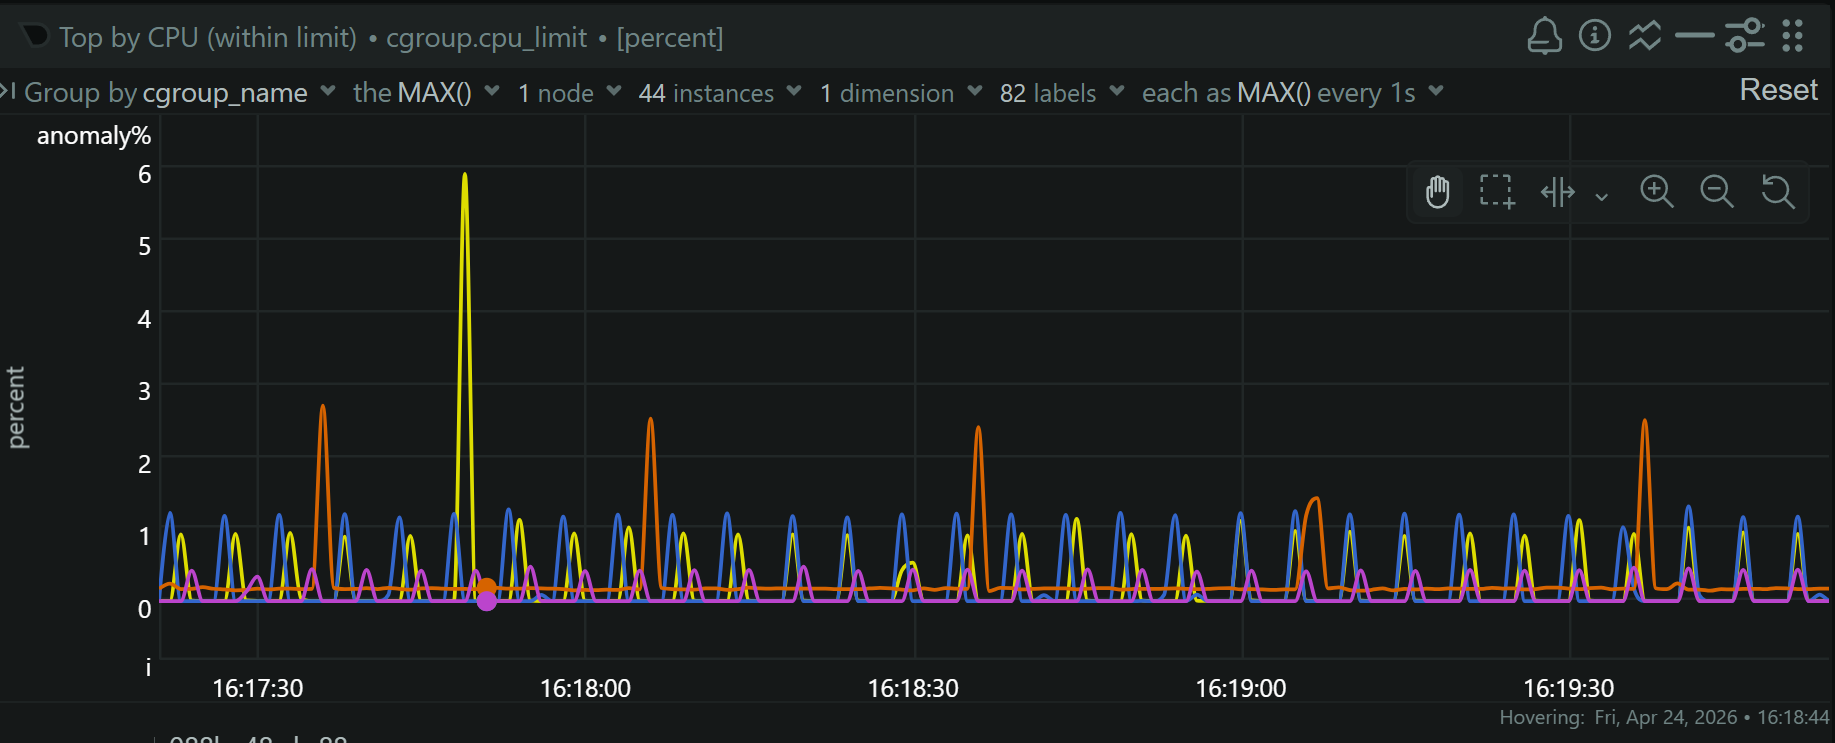
\includegraphics[width=\textwidth]{figuras/capitulo4/4.6/BloqueA/baseline_cpu.png}
    \caption[Consumo de CPU en baseline: cuatro contenedores del \textit{stack}]{Consumo de CPU (\% del límite del cgroup) de los contenedores del \textit{stack} durante parte del período de observación en baseline. Picos máximos: Documenso: 5,9\,\%; Browserless: 2,6\,\%; PostgreSQL: 1,2\,\%; \textit{proxy} Socat: 0,43\,\%.}
    \label{fig:baseline_cpu}
\end{figure}

\FloatBarrier

Los picos de Documenso (máximo 5,9\,\%) correspondieron a solicitudes de renderizado de página y no a procesamiento sostenido. Entre los instantes de actividad, todos los contenedores retornaron a valores próximos a cero. La holgura disponible respecto a los 8~vCPUs del LXC resultó amplia bajo esta carga.

\subsection{Consumo de recursos bajo carga controlada}
\label{subsec:carga_controlada}

Se realizaron dos ensayos de carga sobre el \textit{stack} en producción: el sellado de un documento único y una ráfaga de cinco documentos enviados en intervalos breves.

\subsubsection*{Ensayo 1: sellado de un documento}

Las Figuras~\ref{fig:carga_1firma_cpu} y \ref{fig:carga_1firma_ram} registran el comportamiento del \textit{stack} durante el sellado de un documento individual.

\begin{figure}[!htbp]
    \centering
    \begin{subfigure}[b]{0.95\textwidth}
        \centering
        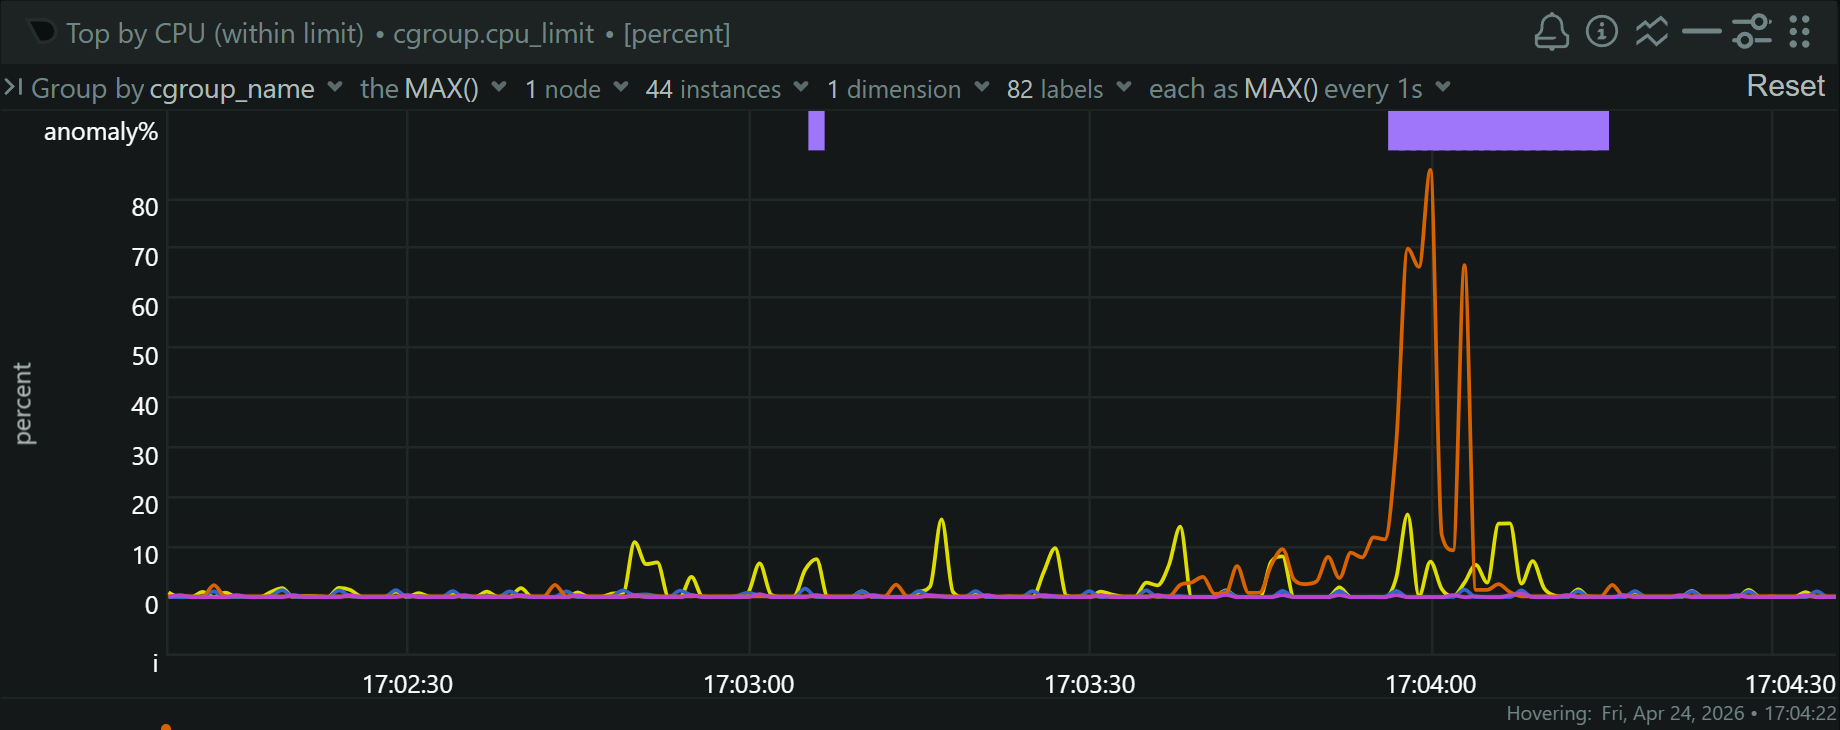
\includegraphics[width=\textwidth]{figuras/capitulo4/4.6/BloqueB/carga_controlada_1firma_cpu.png}
        \caption{Consumo de CPU (\% del límite del cgroup) durante el sellado de un documento. Pico máximo: Browserless 86,00\,\%; Documenso 16,66\,\%.}
        \label{fig:carga_1firma_cpu}
    \end{subfigure}
    \vspace{1em}
    \begin{subfigure}[b]{0.95\textwidth}
        \centering
        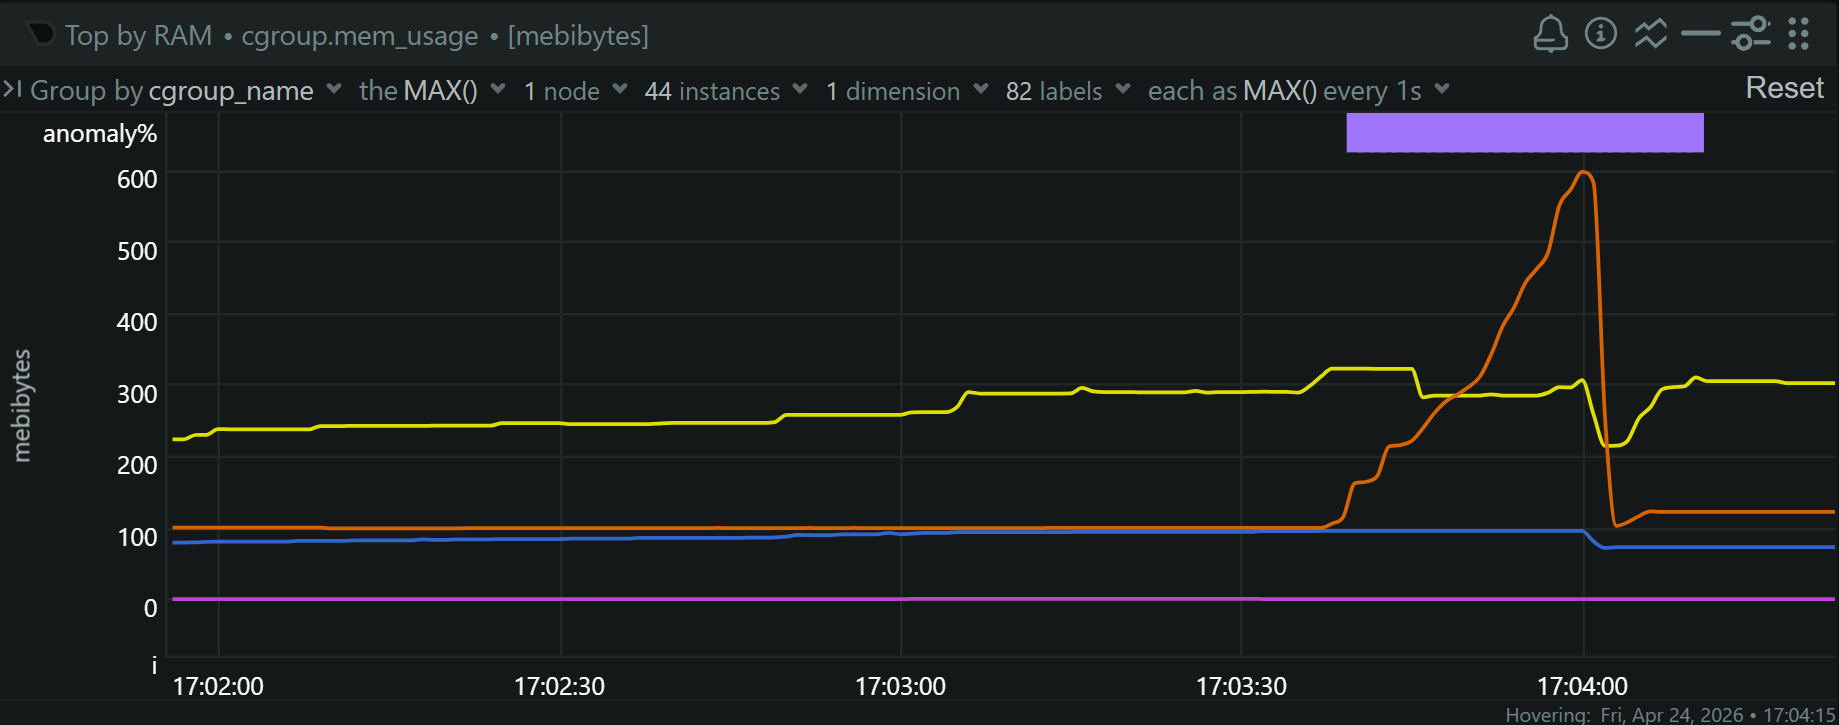
\includegraphics[width=\textwidth]{figuras/capitulo4/4.6/BloqueB/carga_controlada_1firma_ram.png}
        \caption{Consumo de RAM (en MiB) durante el sellado de un documento. Browserless: 102~MiB \(\to\) 600~MiB (pico, +498~MiB), estabilizado en 124,3~MiB (+22,3~MiB retenidos). Documenso: 215,5~MiB \(\to\) 308,8~MiB (+93,3~MiB retenidos). PostgreSQL: pico transitorio de 97~MiB (+20~MiB).}
        \label{fig:carga_1firma_ram}
    \end{subfigure}
    \caption[CPU y RAM durante el sellado de un documento (1 firma)]{Consumo de CPU y RAM del \textit{stack} durante el sellado de un documento. Browserless alcanzó un pico máximo de 86,00\,\% de CPU y 600~MiB de RAM; al concluir el job, la CPU retornó al baseline mientras la RAM se estabilizó en 124,3~MiB. Documenso retuvo 93,3~MiB adicionales de forma permanente tras el evento.}
    \label{fig:carga_1_firma}
\end{figure}

\FloatBarrier

En CPU, el evento se manifestó como un pico aislado de 2~segundos de duración: Browserless alcanzó un máximo de 86,00\,\% mientras Documenso no superó el 16,66\,\%. El resto del \textit{stack} permaneció en valores de baseline. En RAM, Browserless escaló abruptamente desde 102~MiB hasta 600~MiB (+498~MiB) para instanciar el proceso de Chrome encargado del renderizado. Al concluir el job, el proceso fue destruido y el sistema operativo recuperó la memoria; Browserless se estabilizó en 124,3~MiB (+22,3~MiB sobre su baseline) y Documenso en 308,8~MiB (+93,3~MiB). El impacto sobre PostgreSQL fue transitorio (pico de 97~MiB, +20~MiB) y retornó a su valor de baseline al concluir el job.

\subsubsection*{Ensayo 2: ráfaga de cinco documentos}

Las Figuras~\ref{fig:carga_5firmas_cpu} y \ref{fig:carga_5firmas_ram} registran el comportamiento del \textit{stack} durante la ráfaga concurrente.

\begin{figure}[!htbp]
    \centering
    \begin{subfigure}[b]{0.95\textwidth}
        \centering
        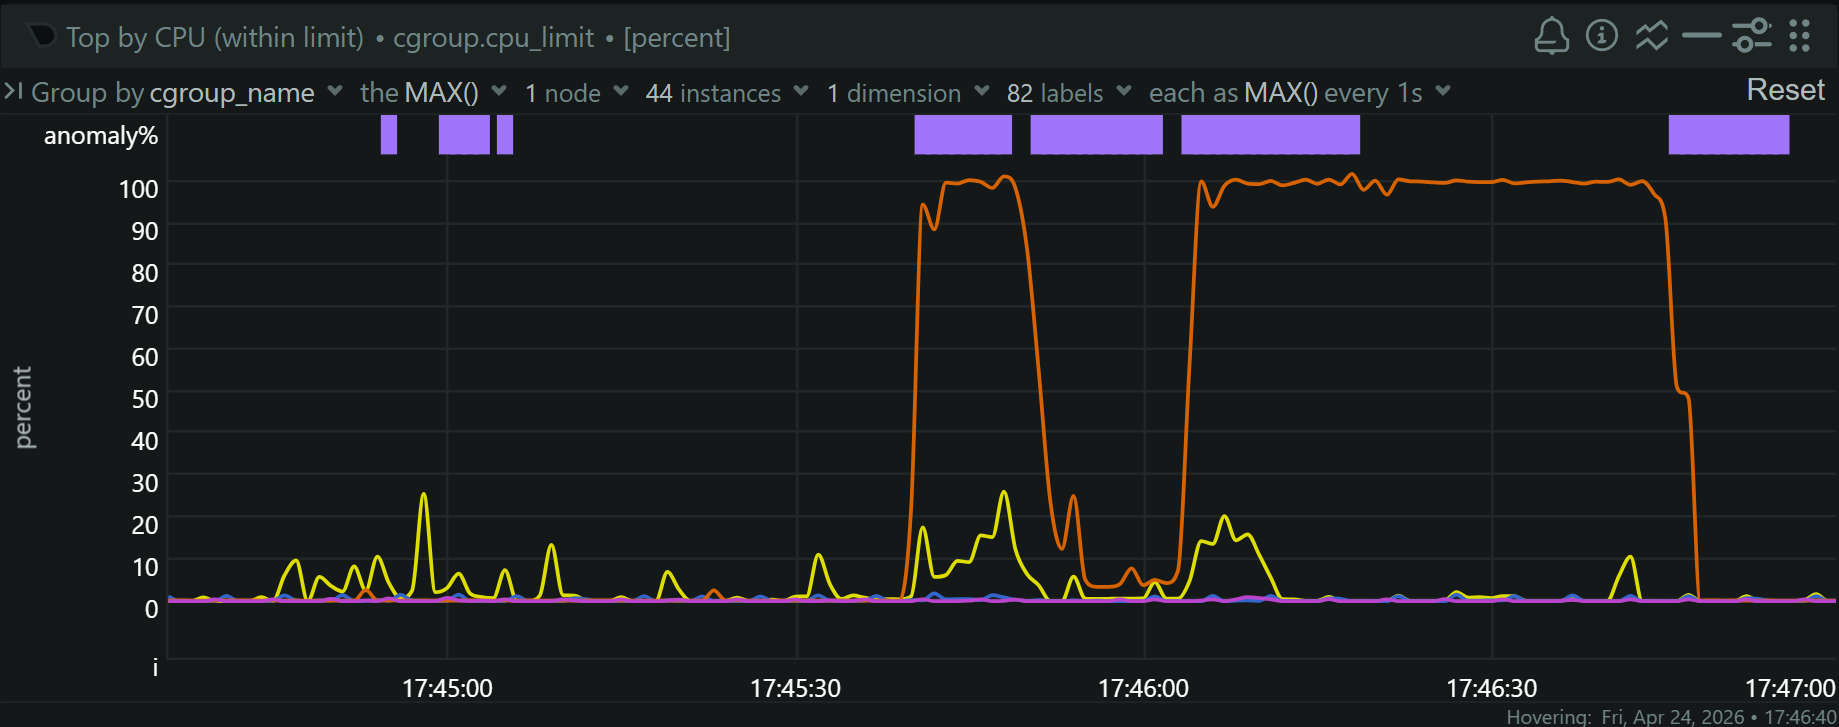
\includegraphics[width=\textwidth]{figuras/capitulo4/4.6/BloqueB/cpu_bajo_carga_controlada_5firmas.png}
        \caption{Consumo de CPU (\% del límite del cgroup) durante la ráfaga de cinco documentos. Pico máximo sostenido: Browserless 100\,\%; Documenso 25\,\% al inicio del proceso.}
        \label{fig:carga_5firmas_cpu}
    \end{subfigure}
    \vspace{1em}
    \begin{subfigure}[b]{0.95\textwidth}
        \centering
        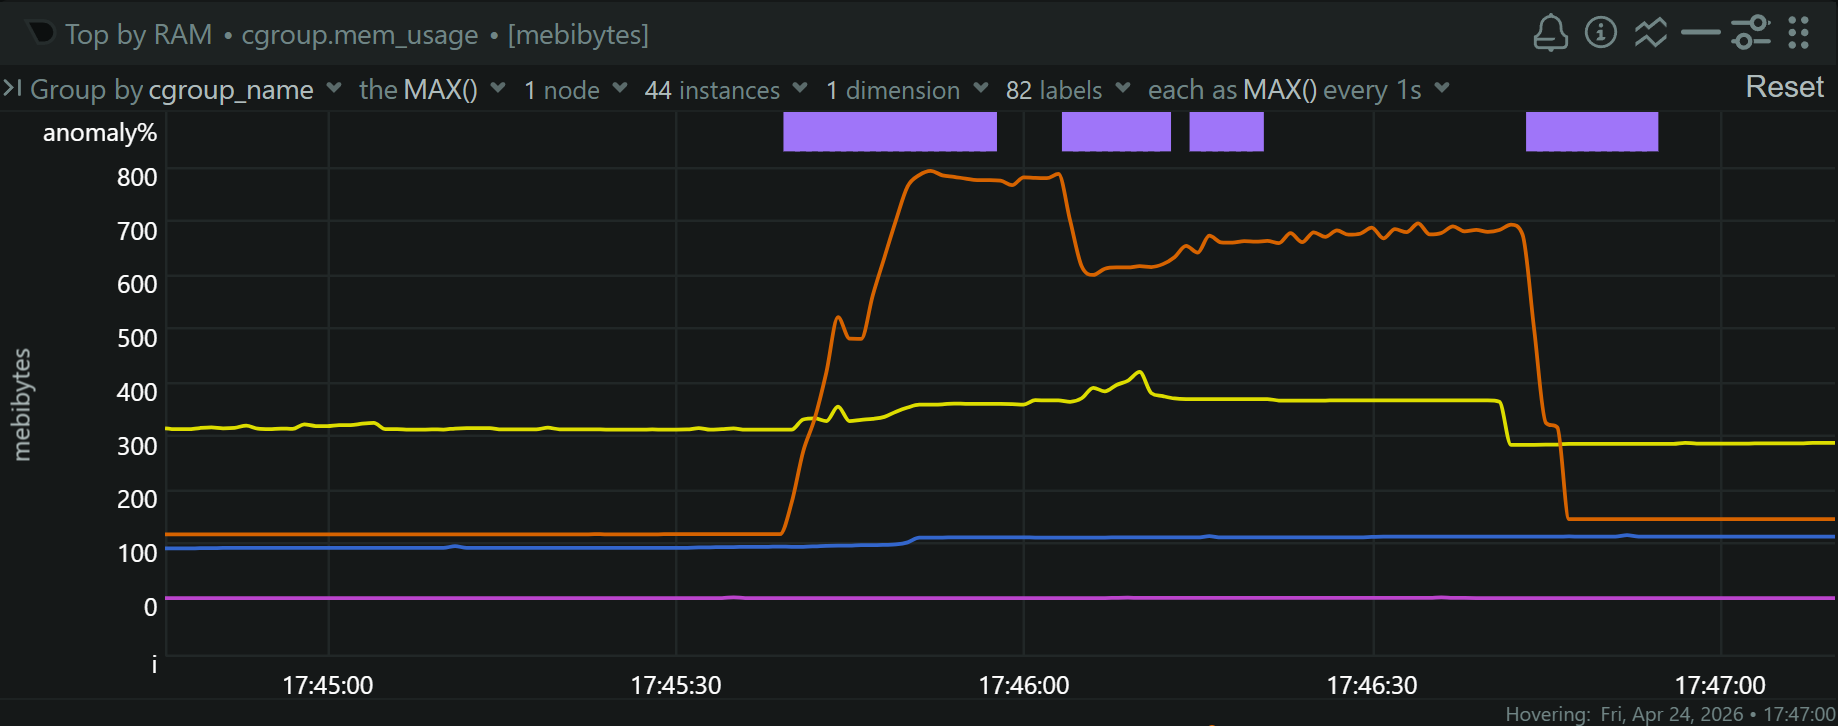
\includegraphics[width=\textwidth]{figuras/capitulo4/4.6/BloqueB/ram_bajo_carga_controlada_5firmas.png}
        \caption{Consumo de RAM (en MiB) durante la ráfaga de cinco documentos. Pico máximo de Browserless: 1\,331~MiB. Total del \textit{stack} en el pico: \(\approx\) 1\,826~MiB sobre 8~GiB asignados al LXC.}
        \label{fig:carga_5firmas_ram}
    \end{subfigure}
    \caption[CPU y RAM durante la ráfaga de cinco documentos concurrentes]{Consumo de CPU y RAM del \textit{stack} durante la ráfaga de cinco documentos. La ventana de actividad se extendió entre las 00:46:28 y las 00:47:40 UTC (\(\approx\)~1~min 12~s). Browserless alcanzó un pico sostenido de 100\,\% de CPU y un pico de RAM de 1\,331~MiB antes de liberar ambos recursos al completarse todos los jobs.}
    \label{fig:carga_5_firmas}
\end{figure}

\FloatBarrier

En este ensayo, el bloque de actividad se extendió entre las 00:46:28 y las 00:47:40 UTC, aproximadamente 1~minuto 12~segundos: Browserless procesó los cinco jobs en forma secuencial, lo que explica la forma escalonada de la curva de RAM (Figura~\ref{fig:carga_5firmas_ram}), donde cada peldaño corresponde al lanzamiento de un proceso de Chrome adicional. El pico máximo de RAM de Browserless fue de 1\,331~MiB. Al completarse el último job, la curva cayó a los 298~MiB de baseline en un único intervalo de muestreo.

En CPU, Browserless registró un pico agudo inicial de 100\,\% a las 00:46:28, un breve descenso hacia el baseline a las 00:46:32 y luego una actividad sostenida al 100\,\% durante aproximadamente 1~minuto hasta las 00:47:38. El pico de 100\,\% corresponde a 1 núcleo virtual sobre los 8~vCPUs del LXC (el 12,5\,\% de la capacidad total). Documenso registró un pico de 25\,\% al inicio del proceso, asociado al despacho inicial de los jobs de sellado, retornando luego al baseline.

\subsubsection*{Tabla comparativa de rendimiento}

La Tabla~\ref{tab:metricas_rendimiento} consolida los valores registrados en ambas subsecciones frente a la capacidad auditada del LXC.

\begin{table}[!htbp]
    \centering
    \caption[Métricas de rendimiento: baseline vs.\ pico bajo carga]{Comparativa de consumo de recursos en baseline y bajo carga controlada (ráfaga de 5 documentos). El límite total del LXC es de 8~vCPUs y 8\,192~MiB de RAM.}
    \label{tab:metricas_rendimiento}
    \begin{tabular}{l r r r}
        \toprule
        \textbf{Componente} & \textbf{Baseline} & \textbf{Pico (ráfaga)} & \textbf{Impacto sobre LXC} \\
        \midrule
        \multicolumn{4}{l}{\textbf{Uso de CPU} (capacidad total: 8~vCPUs)} \\
        \quad Browserless   & 2,6\,\%    & 100\,\%              & \(\approx\) 12,5\,\% (\(\approx\) 1~vCPU) \\
        \quad Documenso     & 5,9\,\%    & 25\,\%   & \(\approx\) 3,1\,\% (\(\approx\) 0,25~vCPU) \\
        \midrule
        \multicolumn{4}{l}{\textbf{Uso de RAM} (capacidad total: 8\,192~MiB)} \\
        \quad Browserless             & \(\approx\) 102,0~MiB  & \(\approx\) 1\,331~MiB & \(\approx\) 16\,\% \\
        \quad \textbf{\textit{Stack} total}    & \textbf{\(\approx\) 396,7~MiB (5\,\%)} & \textbf{\(\approx\) 1\,826~MiB} & \textbf{\(\approx\) 22\,\%} \\
        \bottomrule
    \end{tabular}
\end{table}

\FloatBarrier

El recurso con mayor variación bajo carga fue la RAM de Browserless, que se multiplicó por \(\approx\)~13 respecto al baseline. Aun en el peor caso registrado, el \textit{stack} consumió el 22\,\% de la RAM del LXC, lo que dejó un margen de aproximadamente 6\,366~MiB (\(\approx\) 6,2~GiB) disponibles. La CPU no representó un cuello de botella en ninguno de los dos ensayos.

\section{Validación del Respaldo y Recuperación}
\label{sec:validacion_respaldo}

Esta sección verifica la capa de continuidad definida en la Sección~\ref{sec:metodologia_validacion}: los mecanismos de respaldo automático configurados en la Sección~\ref{sec:estrategia_respaldo_retencion} del Capítulo~\ref{chap:diseno_implementacion} generan y persisten los artefactos esperados en el almacenamiento externo. La validación se apoya en la inspección del \textit{bucket} de MinIO y en los metadatos de los objetos almacenados; el procedimiento operativo de restauración se documenta en el Apéndice~\ref{AppendixC}.

\subsection{Respaldo de la base de datos}
\label{subsec:validacion_respaldo_bd}

El \textit{job} de respaldo de PostgreSQL fue configurado en Coolify para ejecutarse diariamente a las 03:00 y persistir los volcados en el \textit{bucket} \texttt{documenso-backup-databases} del servidor MinIO. La Figura~\ref{fig:minio_bucket_bd_backups} muestra el contenido del bucket al 14 de abril de 2026.

\begin{figure}[!htbp]
    \centering
    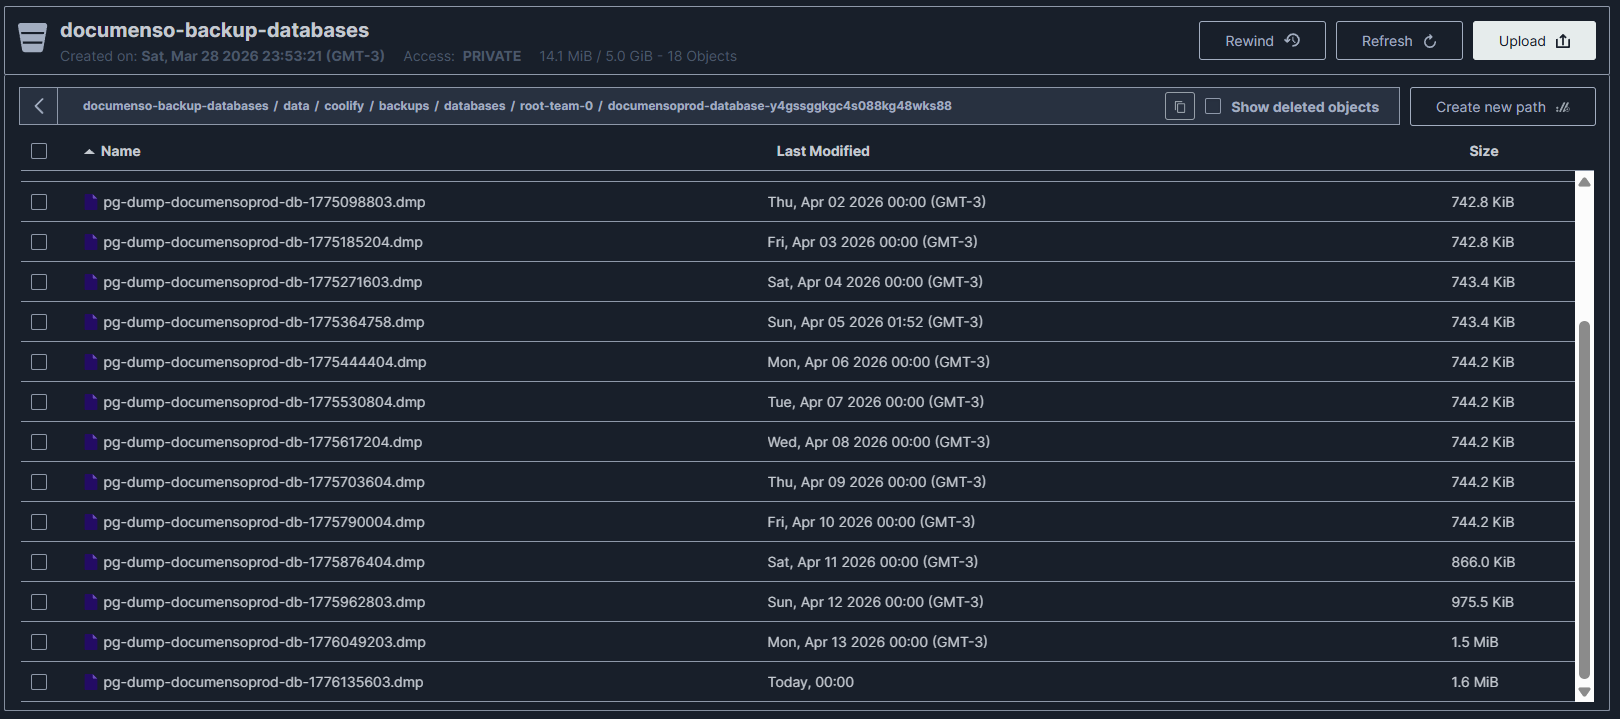
\includegraphics[width=\textwidth]{figuras/capitulo4/4.7/bucket_documenso-backup-databases.png}
    \caption[\textit{Bucket} \texttt{documenso-backup-databases}: listado de volcados diarios de PostgreSQL]{Consola de MinIO mostrando el \textit{bucket} \texttt{documenso-backup-databases}. Se registran 18 objetos con nomenclatura \texttt{pg-dump-documensoprod-db-\{timestamp\}.dmp}, generados diariamente desde el 28 de marzo de 2026. El tamaño total de los artefactos es de 14,1~MiB.}
    \label{fig:minio_bucket_bd_backups}
\end{figure}

\FloatBarrier

El listado registra 18 volcados con una cadencia estrictamente diaria: la marca de tiempo UNIX incluida en cada nombre de archivo garantiza la unicidad del artefacto e impide colisiones de nombres ante reinicios del \textit{job}. Los volcados se almacenan bajo una ruta que contiene el identificador único del contenedor de base de datos.

El tamaño de los artefactos refleja el crecimiento orgánico de la base de datos: los volcados del 2 al 10 de abril se mantuvieron en el rango de 742--744~KiB, período que coincide con el despliegue inicial sin carga de documentos. A partir del 11 de abril, coincidiendo con los ensayos de firma documentados en la Sección~\ref{sec:validacion_e2e}, el tamaño escaló progresivamente hasta 1,6~MiB al 14 de abril, lo que evidencia que cada ciclo de firma incorporó registros nuevos a la base de datos.

La validación de retención para este dominio se realizó mediante inspección directa de metadatos sobre un volcado generado el 7 de abril dentro del \textit{bucket} \texttt{documenso-backup-databases}. En ese objeto, el atributo \texttt{X-\allowbreak Amz-\allowbreak Object-\allowbreak Lock-\allowbreak Mode} registró el valor \texttt{GOVERNANCE} y el atributo \texttt{X-\allowbreak Amz-\allowbreak Object-\allowbreak Lock-\allowbreak Retain-\allowbreak Until-\allowbreak Date} fijó el vencimiento para el 7 de mayo de 2026. Esta evidencia confirma una retención efectiva de 30~días, consistente con la política definida en la Sección~\ref{sec:estrategia_respaldo_retencion}.

\subsection{Prueba de restauración de la base de datos}
\label{subsec:validacion_restauracion_bd}

Se ejecutó un simulacro de restauración a partir de uno de los volcados almacenados en el bucket \texttt{documenso-backup-databases}. Coolify orquestó el comando \texttt{pg\_restore -{}-clean} sobre el contenedor de PostgreSQL, lo que forzó el reemplazo completo del estado previo de la base de datos. La integridad del resultado se verificó accediendo a la aplicación y confirmando que los registros de documentos y firmantes se encontraban íntegros. El procedimiento detallado para importar y restaurar los respaldos se documenta en el Apéndice~\ref{AppendixC:RestauracionBD}.

\subsection{Respaldo de la configuración del \textit{stack}}
\label{subsec:validacion_respaldo_config}

El \textit{script} \texttt{backup-coolify.sh}, configurado mediante \textit{cron} para ejecutarse diariamente a las 04:00, empaqueta los manifiestos y secretos del despliegue y transfiere el resultado al \textit{bucket} \texttt{backups-coolify} de MinIO. La Figura~\ref{fig:minio_bucket_config_backups} muestra el contenido del bucket al 14 de abril de 2026.

\begin{figure}[!htbp]
    \centering
    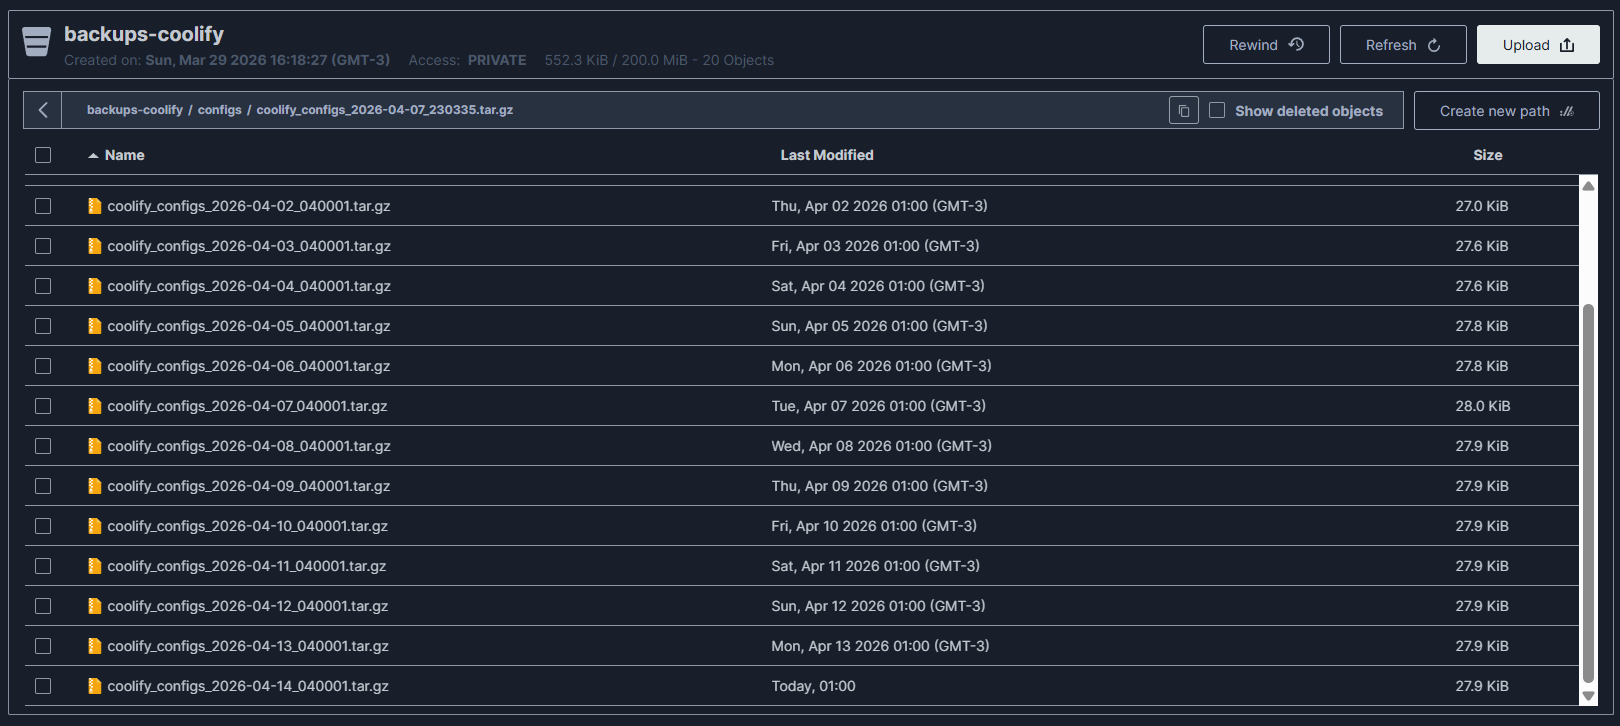
\includegraphics[width=\textwidth]{figuras/capitulo4/4.7/respaldo_configuracion.png}
    \caption[\textit{Bucket} \texttt{backups-coolify}: listado de respaldos diarios de configuración]{Consola de MinIO mostrando el \textit{bucket} \texttt{backups-coolify}. Se registran 20 objetos con nomenclatura \texttt{coolify\_configs\_YYYY-MM-DD\_HHmmss.tar.gz}, generados diariamente desde el 28 de marzo de 2026. El tamaño total de los artefactos es de 552,3~KiB.}
    \label{fig:minio_bucket_config_backups}
\end{figure}

\FloatBarrier

Los 20 artefactos presentan un tamaño estable en el rango de 27,0--28,0~KiB, lo que indica que las configuraciones del conjunto de todos los proyectos administrados por Coolify (incluyendo Documenso) se mantuvieron sin variaciones significativas. La inspección interna del archivo confirmó la presencia de los manifiestos \texttt{docker-compose.yml} y los secretos \texttt{.env} correspondientes, garantizando que el respaldo contiene la información suficiente para reconstruir el entorno ante un escenario de recuperación de desastres. El procedimiento de inspección y extracción de estos respaldos se detalla en el Apéndice~\ref{AppendixC}.

En el dominio de configuraciones, la comprobación se efectuó sobre un respaldo del 7 de abril almacenado en el \textit{bucket} \texttt{backups-coolify}. La lectura de metadatos mostró nuevamente \texttt{X-\allowbreak Amz-\allowbreak Object-\allowbreak Lock-\allowbreak Mode=\allowbreak GOVERNANCE}, mientras que \texttt{X-\allowbreak Amz-\allowbreak Object-\allowbreak Lock-\allowbreak Retain-\allowbreak Until-\allowbreak Date} proyectó la retención hasta el 4 de octubre de 2026. Esta combinación valida que la política aplicada en este dominio corresponde a 180~días. El procedimiento de restauración del \textit{stack} a partir de estos artefactos se documenta en el Apéndice~\ref{AppendixC:RestauracionConfig}.

\subsection{Validación de las políticas de ciclo de vida}
\label{subsec:validacion_ilm}

Las políticas de ciclo de vida configuradas en la Sección~\ref{sec:estrategia_respaldo_retencion} del Capítulo~\ref{chap:diseno_implementacion} se verificaron mediante el comando \texttt{mc ilm ls} del cliente de MinIO, ejecutado sobre cada uno de los tres \textit{buckets} del sistema. Esta verificación es crítica porque, aunque la aplicación no explota versiones de objetos en su operación diaria, la activación de \textit{Object Lock} fuerza el versionado a nivel de infraestructura. En este contexto, la salida del comando demuestra que el motor ILM opera como mecanismo de \textit{Garbage Collection} para purgar \textit{Delete Markers} y evitar el colapso de las cuotas de almacenamiento. La Figura~\ref{fig:minio_ilm_policies} presenta la salida del comando.

Las reglas registradas son coherentes con el diseño: el \textit{bucket} documental (\texttt{documenso-prod}) conserva la versión vigente de cada objeto durante 1\,825~días (cinco años) y elimina las versiones anteriores tras un día, mientras que los \textit{buckets} de respaldo aplican retenciones de 30 y 180~días respectivamente. En los tres casos, el campo \texttt{KEEP VERSIONS} registra el valor 0, lo que indica que las versiones no vigentes no se acumulan más allá del plazo configurado.

\begin{figure}[!htbp]
    \centering
    \begin{subfigure}[b]{0.85\textwidth}
        \centering
        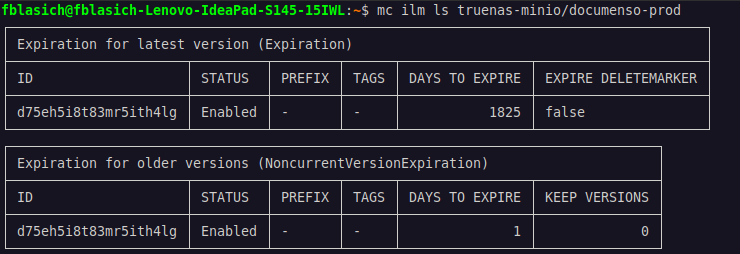
\includegraphics[width=\textwidth]{figuras/capitulo3/documenso-prod_retention-policies.png}
        \caption{\textit{Bucket} \texttt{documenso-prod}: expiración de la versión vigente a los 1\,825~días y eliminación de versiones anteriores tras 1~día.}
        \label{fig:ilm_documenso_prod}
    \end{subfigure}
    \vspace{0.5em}
    \begin{subfigure}[b]{0.85\textwidth}
        \centering
        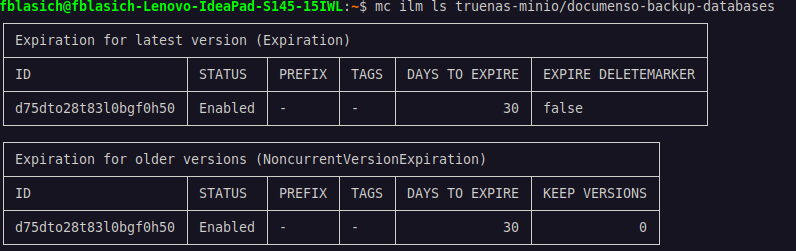
\includegraphics[width=\textwidth]{figuras/capitulo3/documenso-backup-databases_retention-policies.png}
        \caption{\textit{Bucket} \texttt{documenso-backup-databases}: expiración y eliminación de versiones anteriores a los 30~días.}
        \label{fig:ilm_documenso_db_backups}
    \end{subfigure}
\end{figure}
\begin{figure}[!htbp]
    \ContinuedFloat
    \centering
    \begin{subfigure}[b]{0.85\textwidth}
        \centering
        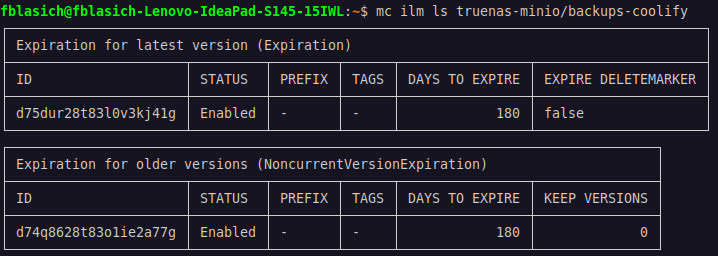
\includegraphics[width=\textwidth]{figuras/capitulo3/backups-coolify_retention-policies.png}
        \caption{\textit{Bucket} \texttt{backups-coolify}: expiración y eliminación de versiones anteriores a los 180~días.}
        \label{fig:ilm_backups_coolify}
    \end{subfigure}
    \caption[Políticas ILM activas en los tres \textit{buckets} del sistema]{Salida del comando \texttt{mc ilm ls} sobre los tres \textit{buckets} del despliegue. Cada regla indica el tipo de transición, el período de retención y el estado activo de la política.}
    \label{fig:minio_ilm_policies}
\end{figure}

\FloatBarrier

La interfaz web de MinIO permite corroborar la configuración de cada \textit{bucket} desde una perspectiva complementaria. La Figura~\ref{fig:minio_ui_buckets} muestra el panel de administración con el estado del versionado, el bloqueo de objetos y la política de retención activa.

\begin{figure}[H]
    \centering
    \begin{subfigure}[b]{0.85\textwidth}
        \centering
        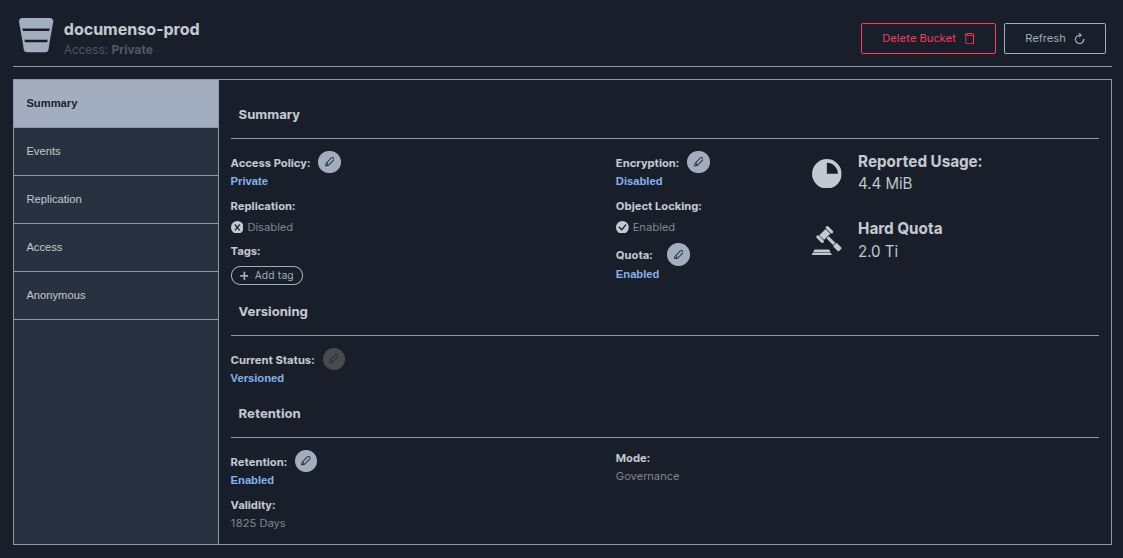
\includegraphics[width=\textwidth]{figuras/capitulo3/documenso-prod.png}
        \caption{\textit{Bucket} \texttt{documenso-prod}: Object Locking habilitado, versionado activo, retención Governance de 1\,825~días, cuota de 2,0~TiB.}
        \label{fig:minio_ui_documenso_prod}
    \end{subfigure}
\end{figure}

\begin{figure}[H]
    \ContinuedFloat
    \centering
    \begin{subfigure}[b]{0.85\textwidth}
        \centering
        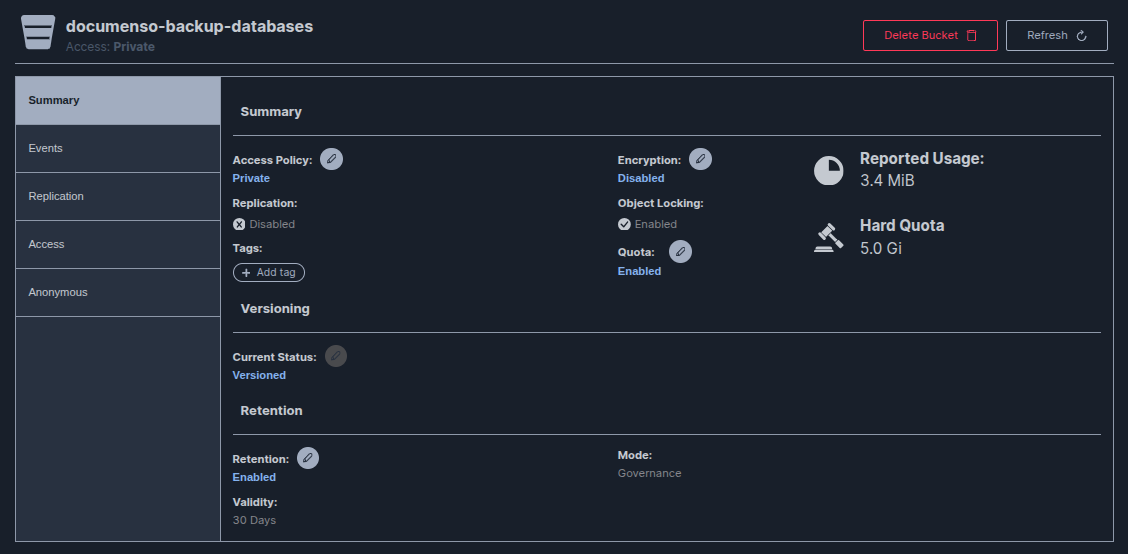
\includegraphics[width=\textwidth]{figuras/capitulo3/documenso-backup-databases.png}
        \caption{\textit{Bucket} \texttt{documenso-backup-databases}: Object Locking habilitado, versionado activo, retención Governance de 30~días, cuota de 5,0~GiB.}
        \label{fig:minio_ui_documenso_db_backups}
    \end{subfigure}
    
    \vspace{0.5em}
    
    \begin{subfigure}[b]{0.85\textwidth}
        \centering
        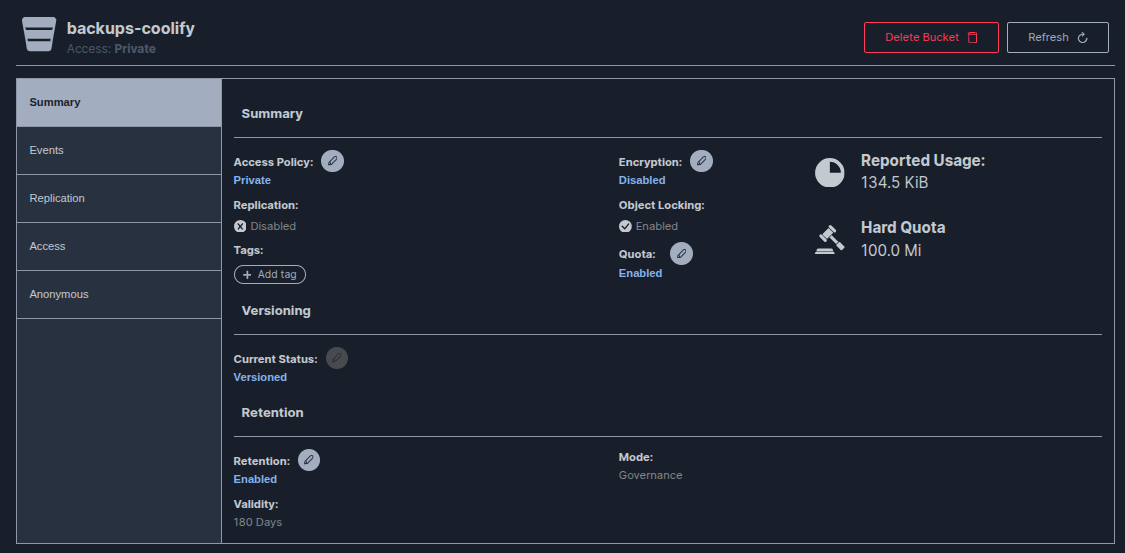
\includegraphics[width=\textwidth]{figuras/capitulo3/backups-coolify.png}
        \caption{\textit{Bucket} \texttt{backups-coolify}: Object Locking habilitado, versionado activo, retención Governance de 180~días, cuota de 100,0~MiB.}
        \label{fig:minio_ui_backups_coolify}
    \end{subfigure}
    \caption[Interfaz web de MinIO: configuración de los tres \textit{buckets} del sistema]{Panel de administración de MinIO para los tres \textit{buckets} del despliegue. Se observan el estado del versionado, el bloqueo de objetos, la política de retención y la cuota asignada.}
    \label{fig:minio_ui_buckets}
\end{figure}

\FloatBarrier

Los resultados confirman que las tres capas de protección ---reglas ILM, bloqueo de objetos en modo Governance y cuotas de almacenamiento--- se encuentran activas y operativas en cada \textit{bucket} del sistema.

\section{Trazabilidad y Cumplimiento de Requisitos}
\label{sec:trazabilidad}

Esta sección cierra el ciclo de validación. La
Tabla~\ref{tab:trazabilidad} vincula cada requisito del alcance definido en el
Capítulo~\ref{chap:introduccion} con la sección del
Capítulo~\ref{chap:diseno_implementacion} donde fue abordado y con la evidencia
empírica que lo valida. A continuación, la Tabla~\ref{tab:comparativa_final} retoma
el análisis del estado del arte para contrastar las condiciones de las plataformas
comerciales con los resultados de la infraestructura desplegada.

\subsection{Matriz de trazabilidad}
\label{subsec:trazabilidad_requisitos}

\small
\begin{longtable}{p{3.8cm} p{1.6cm} p{1.6cm} p{5.2cm}}
    \caption[Matriz de trazabilidad de requisitos]{Trazabilidad entre los requisitos
    del Capítulo~\ref{chap:introduccion}, el diseño del
    Capítulo~\ref{chap:diseno_implementacion} y la validación del presente capítulo.
    Las columnas ``Diseño'' y ``Validación'' indican el número de la sección
    correspondiente.}
    \label{tab:trazabilidad} \\
    \toprule
    \textbf{Requisito} &
    \textbf{Diseño} &
    \textbf{Validación} &
    \textbf{Resultado} \\
    \midrule
    \endfirsthead
    \multicolumn{4}{c}{\tablename\ \thetable{} -- \textit{Continuación de la página anterior}} \\
    \toprule
    \textbf{Requisito} &
    \textbf{Diseño} &
    \textbf{Validación} &
    \textbf{Resultado} \\
    \midrule
    \endhead
    \midrule
    \multicolumn{4}{r}{\textit{Continúa en la siguiente página}} \\
    \endfoot
    \bottomrule
    \endlastfoot
    Selección de plataforma de código abierto &
    \ref{sec:configuracion_servicios} &
    \ref{sec:validacion_e2e} &
    Cumplido. Flujo \textit{end-to-end} validado con usuarios reales. \\
    \addlinespace
    Despliegue contenerizado sobre infraestructura institucional (Proxmox, Coolify) &
    \ref{sec:infraestructura_base} &
    \ref{sec:validacion_despliegue} &
    Cumplido. Estado \textit{Healthy} alcanzado; restricción AVX mitigada. \\
    \addlinespace
    Autenticación restringida al dominio institucional &
    \ref{subsec:google_oauth} &
    \ref{sec:validacion_acceso} &
    Cumplido. Acceso institucional validado; dominios externos bloqueados con
    \texttt{403}. \\
    \addlinespace
    Integración con almacenamiento de objetos (MinIO) mediante \textit{proxy} Socat &
    \ref{sec:proxy_socat} &
    \ref{subsec:validacion_minio} &
    Cumplido. Lectura y escritura por túnel TCP con \texttt{HTTP 200 OK}. \\
    \addlinespace
    Correo transaccional con entregabilidad verificada (Brevo SMTP) &
    \ref{subsec:brevo_smtp} &
    \ref{subsec:validacion_smtp} &
    Cumplido. SPF, DKIM y DMARC en \textit{pass}; entregabilidad verificada. \\
    \addlinespace
    Firma electrónica con certificado institucional &
    \ref{subsec:documenso_core} &
    \ref{subsec:verificacion_firma_adobe} &
    Cumplido. Sello validado en Adobe Acrobat; limitación de confianza documentada. \\
    \addlinespace
    Estrategia de respaldo y retención de datos &
    \ref{sec:estrategia_respaldo_retencion} &
    \ref{sec:validacion_respaldo} &
    Cumplido. ILM y \textit{Object Lock} activos. \\
    \addlinespace
    Consumo de recursos dentro de la capacidad del LXC &
    \ref{sec:infraestructura_base} &
    \ref{sec:metricas_rendimiento} &
    Cumplido. RAM pico \texttt{22\,\%}; CPU dentro de umbrales operativos. \\
    \addlinespace
    Acceso web \textit{clientless} (usabilidad) &
    \ref{subsec:documenso_core} &
    \ref{sec:ensayos_validacion} &
    Cumplido. Operatividad desde navegadores estándar sin software adicional. \\
    \addlinespace
    Elaboración del manual de mantenimiento &
    N/A &
    Apéndice~\ref{AppendixC:Manual} &
    Cumplido. Procedimientos técnicos de mantenimiento documentados. \\
    \addlinespace
    Elaboración del manual de usuarios &
    N/A &
    Apéndice~\ref{AppendixD} &
    Cumplido. Procedimientos operativos de uso documentados. \\
\end{longtable}
\normalsize

\FloatBarrier

\subsection{Comparativa con el estado del arte}
\label{subsec:comparativa_estado_arte}

La Tabla~\ref{tab:comparativa_final} retoma el análisis de mercado presentado en la
Sección~\ref{sec:estado_arte} del Capítulo~\ref{chap:introduccion} y lo contrasta
con los resultados de la solución implementada. El propósito no es establecer una
superioridad absoluta sobre los proveedores comerciales, sino verificar que la
alternativa de código abierto resolvió los condicionantes que motivaron su adopción
en el contexto institucional de la FACET.

\begin{table}[!htbp]
    \centering
    \small
    \caption[Comparativa final: plataformas \textit{SaaS} versus solución implementada]{Contraste
    entre las condiciones de las plataformas comerciales relevadas en la
    Sección~\ref{sec:estado_arte} y los resultados de la infraestructura desplegada.}
    \label{tab:comparativa_final}
    \begin{tabular}{p{3.4cm} p{4.5cm} p{4.5cm}}
        \toprule
        \textbf{Aspecto} &
        \textbf{Plataformas \textit{SaaS}} &
        \textbf{Solución implementada} \\
        \midrule
        Costo de licenciamiento (20~usuarios) &
        \(\approx\) 5\,326~USD anuales recurrentes &
        Costo de licencia nulo \\
        \addlinespace
        Soberanía de los datos &
        Retención y ubicación dependientes del proveedor &
        \textit{On-Premise} (servidores propios de la UNT) \\
        \addlinespace
        Gestión de identidad &
        SSO condicionado a plan \textit{Enterprise} &
        SSO con Google OAuth~2.0 sin costo \textit{Enterprise} adicional \\
        \addlinespace
        Límites de uso &
        Límites por usuario/año (p.\,ej., 100~documentos) &
        Limitado solo por hardware institucional (2~TB) \\
        \addlinespace
        Inmutabilidad y retención &
        Retención opaca y dependiente de políticas del proveedor &
        Control total mediante \textit{Object Lock} e ILM a nivel de \textit{bucket} \\
        \addlinespace
        Certificado de firma &
        Emitido y administrado por el proveedor &
        Certificado institucional generado y controlado por la FACET \\
        \addlinespace
        Carga operativa y disponibilidad &
        Cubierta por SLA del proveedor &
        Asumida por la institución (\textit{trade-off} operativo) \\
        \bottomrule
    \end{tabular}
\end{table}

\FloatBarrier

La adopción del esquema \textit{On-Premise} implica que el área de TI de la facultad asume
la carga operativa que en los servicios comerciales queda cubierta por contrato.
Como contrapartida, la solución eliminó el costo recurrente de 5\,326~USD anuales
proyectado en el estudio inicial, mantuvo los documentos dentro de la
infraestructura propia de la UNT y integró el acceso al directorio
institucional sin dependencia de un proveedor externo.
